\documentclass[]{article}
\usepackage[utf8]{inputenc}
\usepackage[ngerman]{babel}
\usepackage[T1]{fontenc}
\usepackage{%
	ngerman,
	ae,
	times,  %% hier kann man die Schriftart einstellen
	graphicx,
	url,
	scrlayer-scrpage,
	lastpage,
	mathtools,
	geometry,
	multicol,
	cancel,
	xcolor,
	nicematrix,
	xfrac,
	tikz,
	pgfplots,
	amsmath,
	colortbl,
	centernot,
	dsfont,
	textgreek,
	icomma,
	pdfpages,
	kvmap}
\usepackage[hidelinks]{hyperref}
\usepackage[thinlines]{easybmat}
\usetikzlibrary{datavisualization}
\usetikzlibrary{datavisualization.formats.functions}
\usetikzlibrary{intersections}
\pgfplotsset{compat=1.17}
\newcommand{\del}[1]{\cancel{~#1~}}
\NiceMatrixOptions{ last-col,code-for-last-col = \color{blue}\scriptstyle,light-syntax}
\newlength\dlf
\newcommand\alignedhighlight[3]{
  % #1 = color
  % #2 = before alignment
  % #3 = after alignment
  &
  \begingroup
  \settowidth\dlf{$\displaystyle #2$}
  \addtolength\dlf{\fboxsep+\fboxrule}
  \hspace{-\dlf}
  \fcolorbox{#1}{#1}{$\displaystyle #2 #3$}
  \endgroup
}
\newcommand{\reference}[1]{ \text{\small{\textcolor{blue}{(#1)}}} }

\newcommand{\topic}{Mathematik 1}
\newcommand{\subtopic}{Zusammenfassung}
\newcommand{\authors}{Nils Helming}

%Head and Footnotes
\setlength{\headheight}{2.1\baselineskip} %baselineskip = minimum distance bbetween the bottom of one line to another.
\geometry{bottom = 3cm}
\setlength{\headsep}{\baselineskip}
\ihead[\topic\hrule]{\topic\hrule}
\chead[\subtopic\\~]{\subtopic\\~}
\ohead[\authors\\~]{\authors\\~}
\ifoot[\hyperlink{toc}{Zurück zum Inhaltsverzeichnis}]{\hyperlink{toc}{Zurück zum Inhaltsverzeichnis}}
\cfoot[~]{~}
\ofoot[Seite \thepage~von \pageref{LastPage}]{Seite \thepage~von \pageref{LastPage}}

%Paragraph spacings
\setlength{\parindent}{0em} %em = with of an 'M'
\setlength{\parskip}{1ex} %ex = height of an 'x'


\newcommand{\V}{\lor}
\newcommand{\A}{\land}
\newcommand{\T}[1]{\overline{#1}}
\newcommand{\eq}{\Leftrightarrow}
\newcommand{\rarr}{\Rightarrow}
\newcommand{\red}[1]{\textcolor{red}{#1}}

\newcommand{\unit}[1]{\text{#1}}
\newcommand{\fracunit}[2]{\frac{\unit{#1}}{\unit{#2}}}
\newcommand{\textsq}[1]{\ensuremath{\text{#1}^2}}
\newcommand{\textpow}[2]{\ensuremath{\text{#1}^{#2}}}
\newcommand{\tdot}{\ensuremath{\cdot}}


\begin{document}
\tableofcontents
\addtocontents{toc}{\protect\hypertarget{toc}{}}
\pagebreak
\section{Vorlesung 1 (06.10.2020)}
\subsection{Definition: Menge, Mengenelemente, leere Menge}
\subsection{Venn-Diagramme}
\subsection{Definition: Aussage}
\subsection{Definition: Aussageverknüpfung}
\subsection{Beispiele: Verneinung, Konjunktion, Desjunktion, Implikation, Äquivalenz}
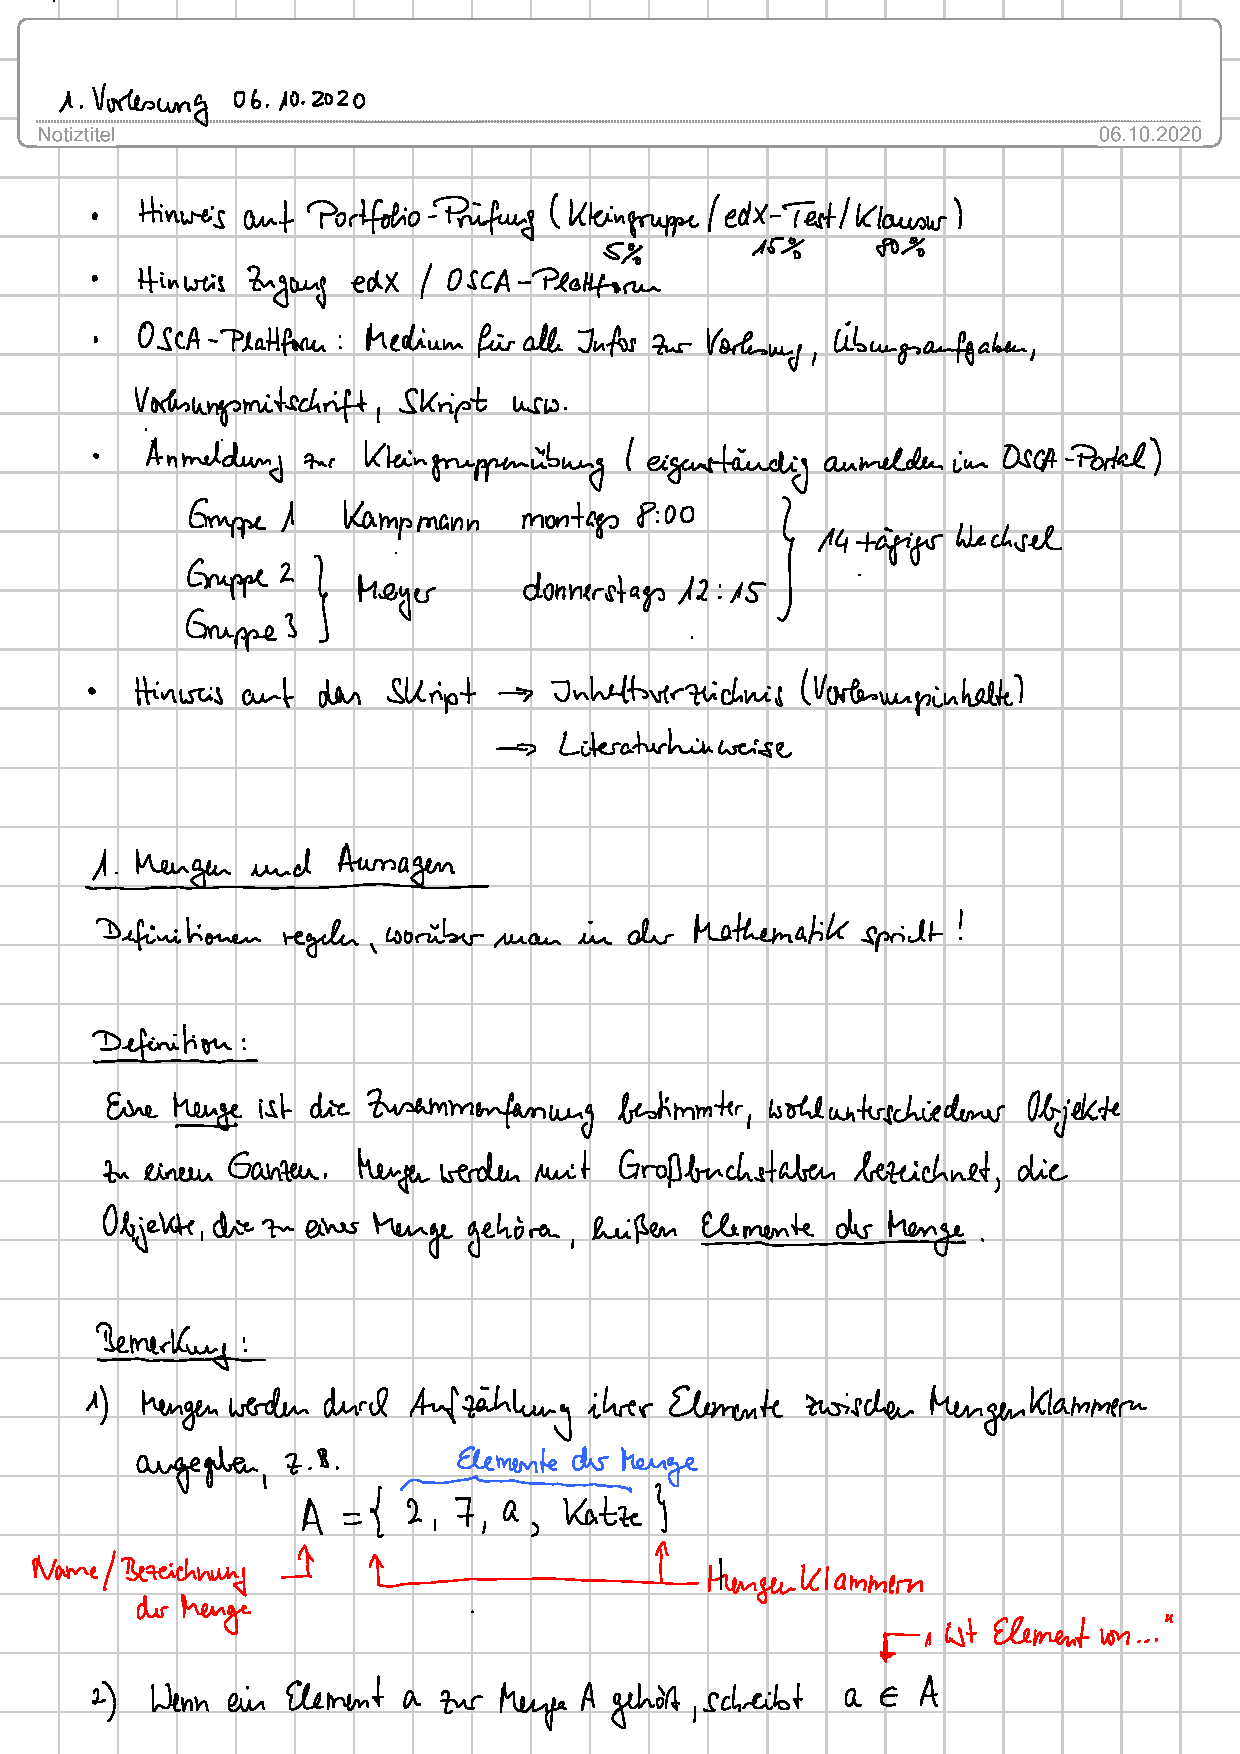
\includepdf[pages=-]{Mitschriften/1. Vorlesung 06.10.2020}

\section{Vorlesung 2 (07.10.2020)}
\subsection{Aussagenlogik: Tautologie, XOR, Allquantor, Existenzquantor}
\subsection{Rechenregeln für Aussageverknüpfung}
\subsection{Axiomatische Mengenlehre (Zermelo-Fraenkel)}
\subsection{Definition: Potenzmenge}
\subsection{Definition: Rechnen mit Mengen - Vereinigung, Durchschnitt, Differenz, Komplement}
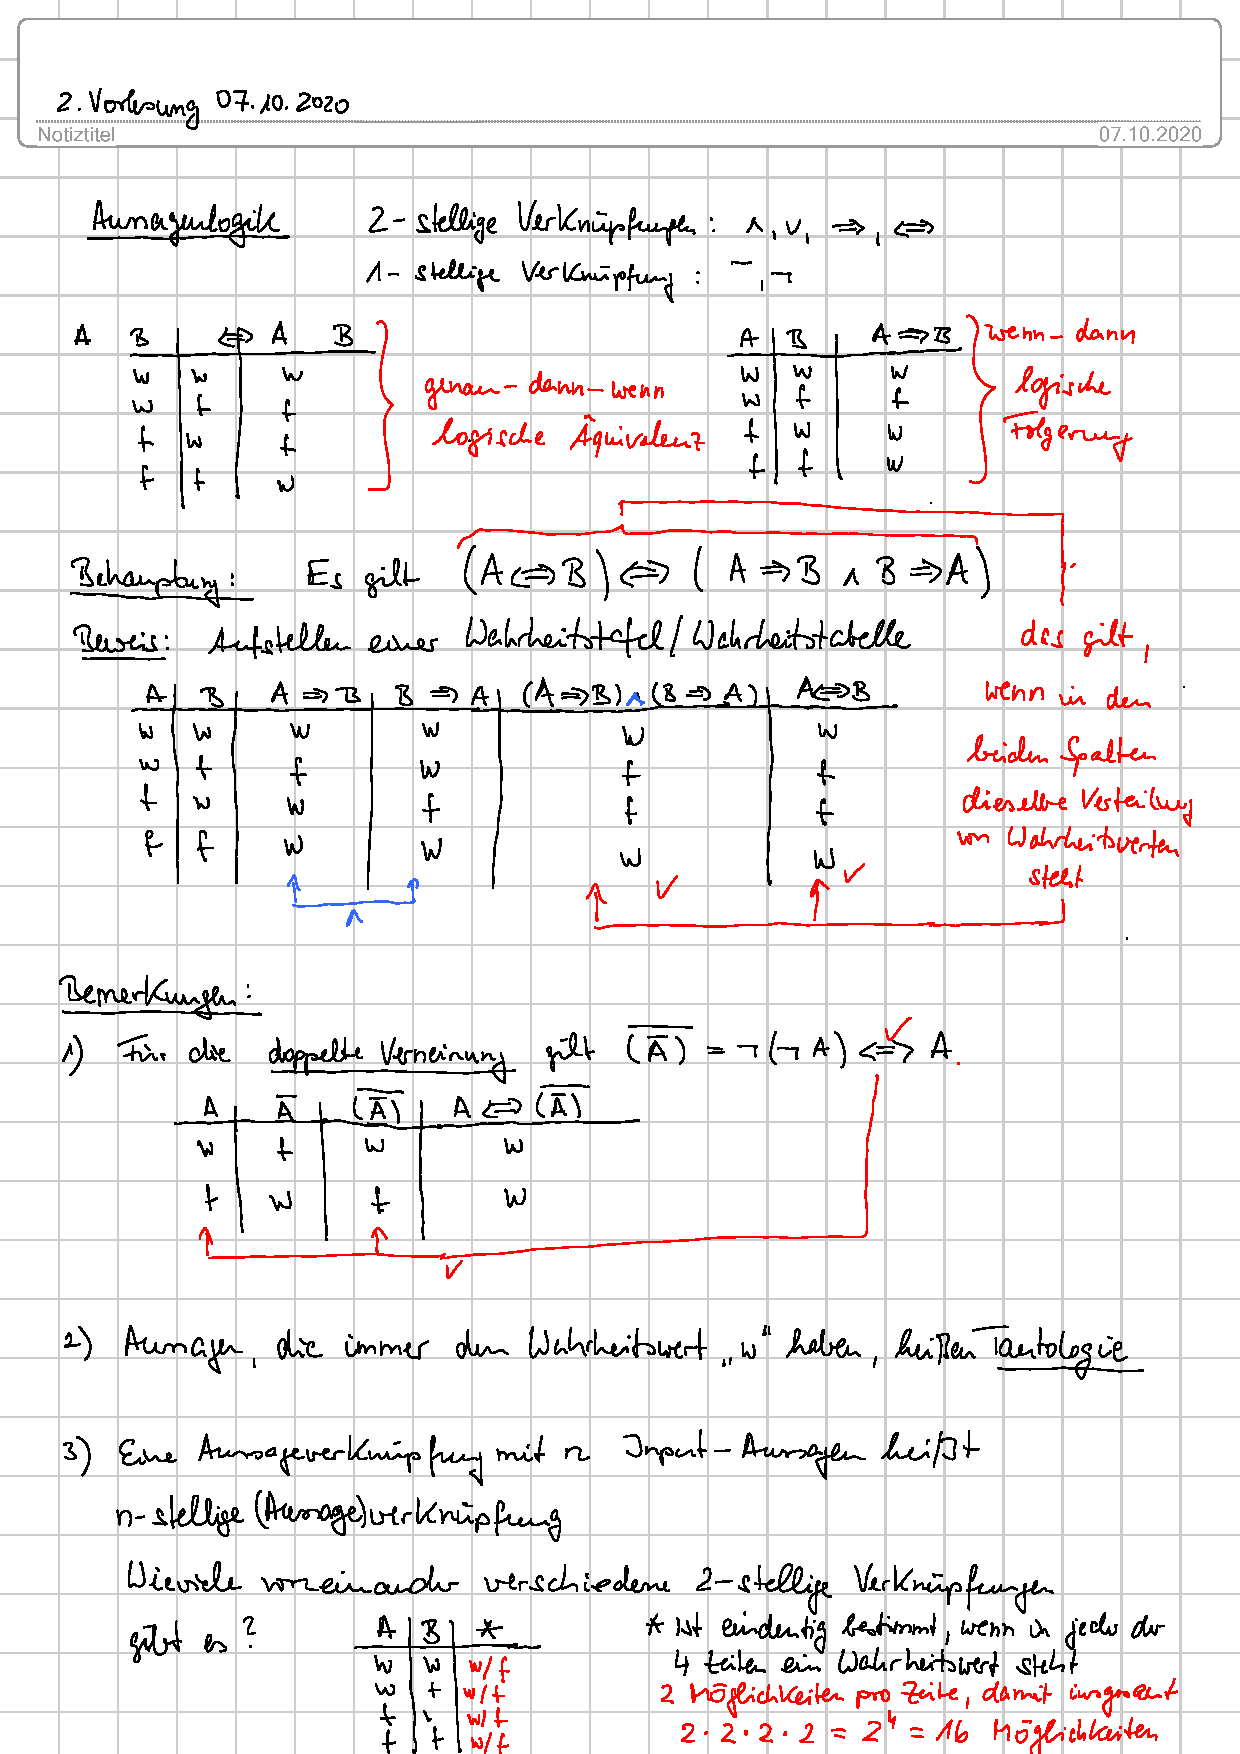
\includepdf[pages=-]{Mitschriften/2. Vorlesung 07.10.2020}

\section{Vorlesung 3 (12.10.2020)}
\subsection{Zahlenmengen}
\subsection{Definition: Aussageform}
\subsection{Definition: Kartesisches Produkt von Mengen, Tupel}
\subsection{Zahlenstrahl, Anordnung von Zahlen}
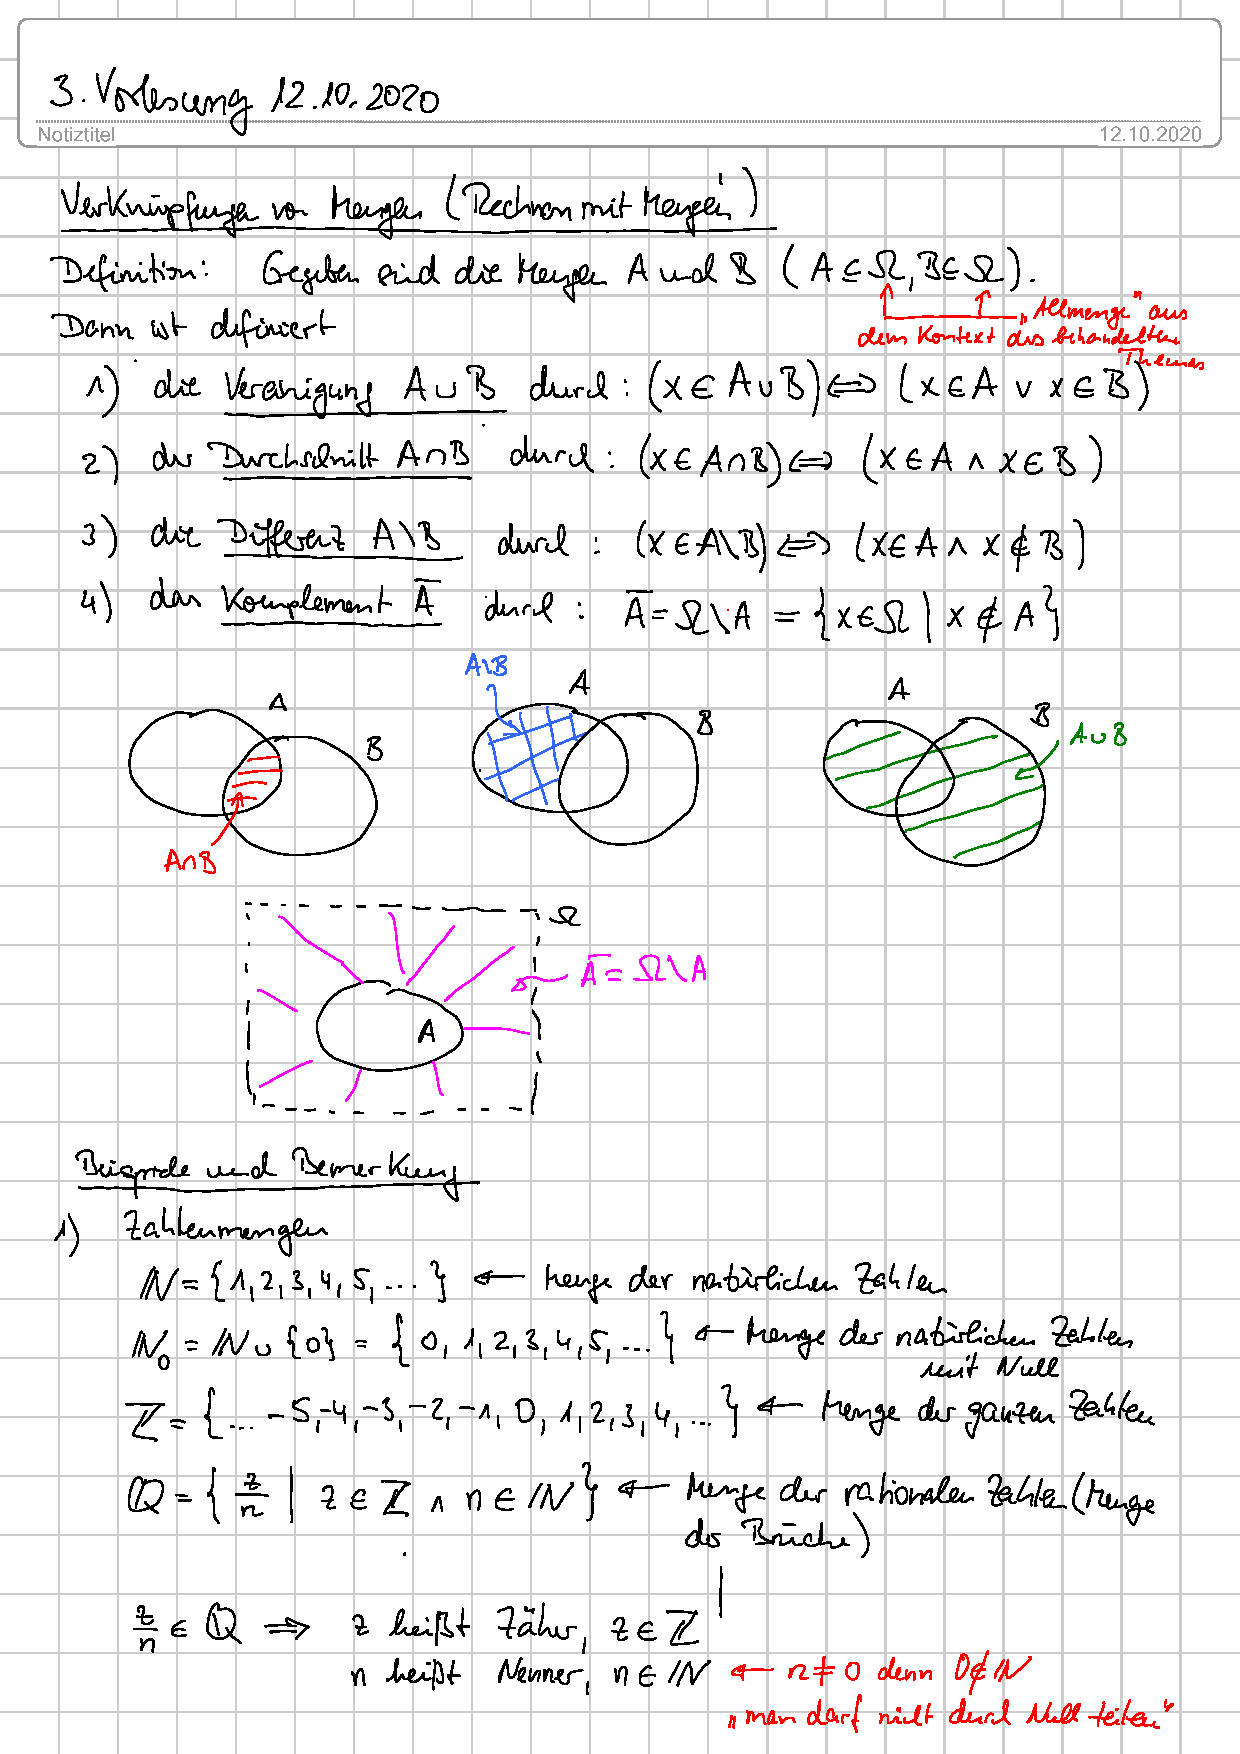
\includepdf[pages=-]{Mitschriften/3. Vorlesung 12.10.2020}

\section{Vorlesung 4 (13.10.2020)}
\subsection{Beipiele Relationen + Kartesisches Produkt}
\subsection{Definition: reflexiv, transitiv, symmetrisch, antisymmetrisch: Äquivalenzrelation, Ordnungsrelation}
\subsection{Definition: Äquivalenzklasse}
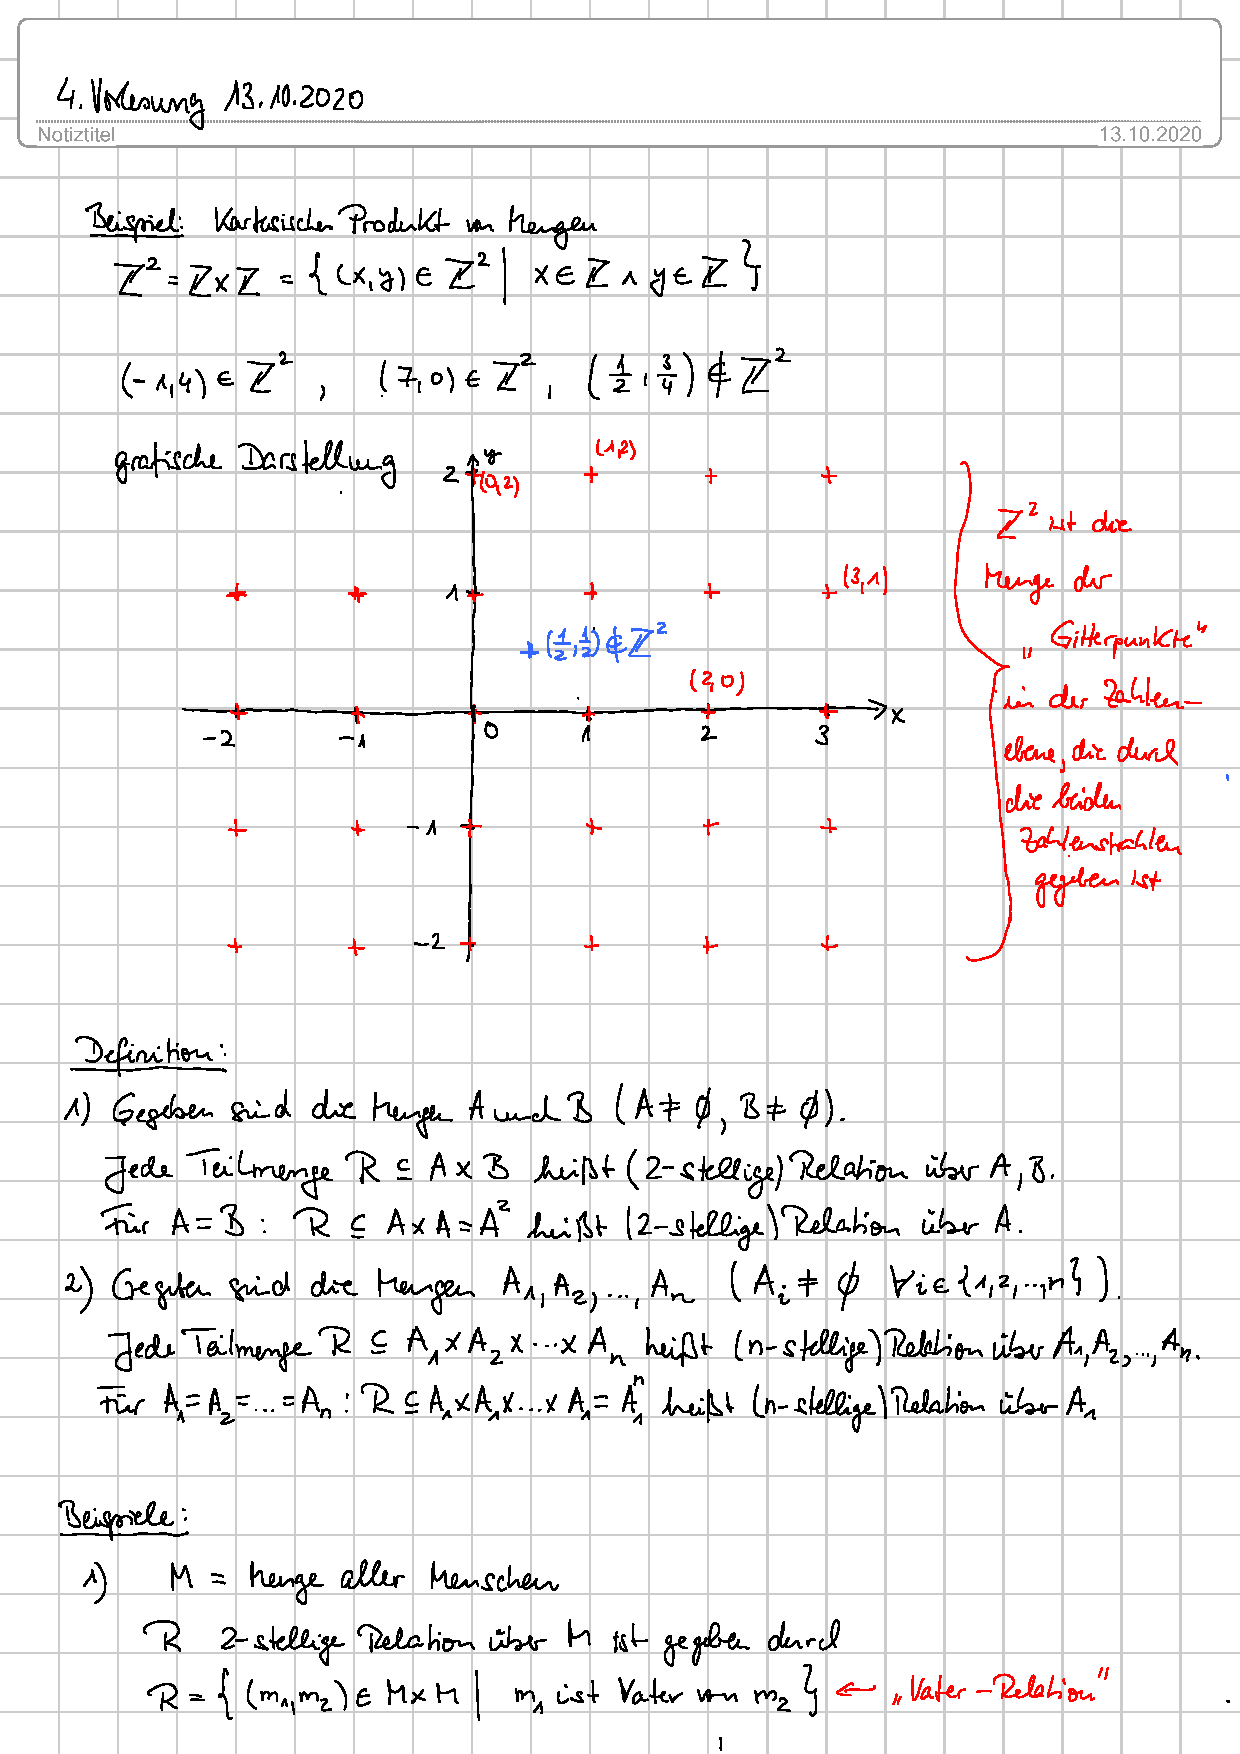
\includepdf[pages=-]{Mitschriften/4. Vorlesung 13.10.2020}

\section{Vorlesung 5 (14.10.2020)}
\subsection{Beipiele Äquivalenzklasse}
\subsection{Definition: vollständige Mengenpartition}
\subsection{Satz: Aquivalenzklassen bilden vollständige Mengenpartition}
\subsection{Definition: Verknüpfung}
\subsection{Definition: Abbildung, Funktion, Bild, Graph, Urbild}
\subsection{grafische Veranschaulichtung der reellen Zahlen}
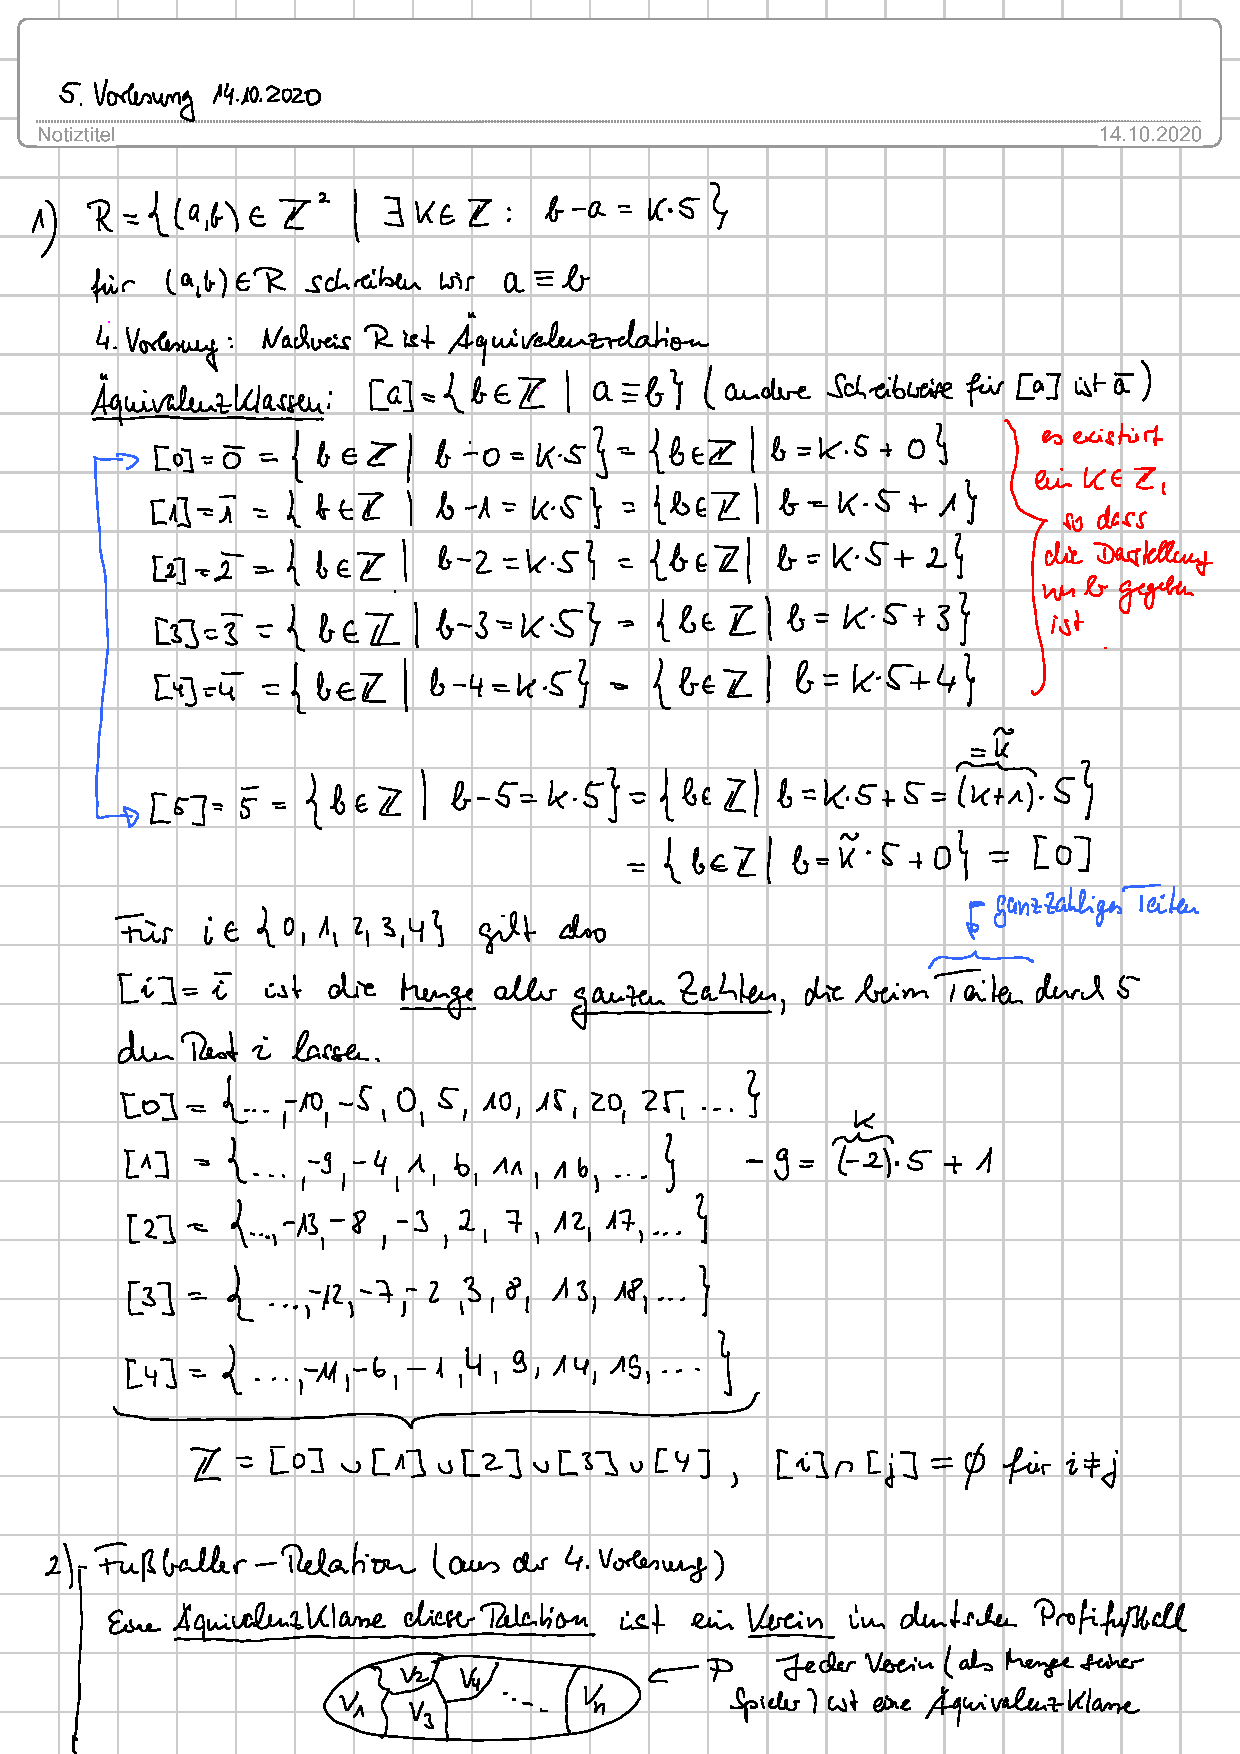
\includepdf[pages=-]{Mitschriften/5. Vorlesung 14.10.2020}

\section{Vorlesung 6 (19.10.2020)}
\subsection{Beipiele Abbildung, Funktion}
\subsection{Zahlensysteme}
\subsection{Peano-Axiome (natürliche Zahlen definieren)}
\subsection{Rechenregeln in den natürlichlen Zahlen}
\subsection{Definition: Endliche Summe}
\subsection{5. Peano-Axiom / Induktionsaxiom / vollständige Induktion}
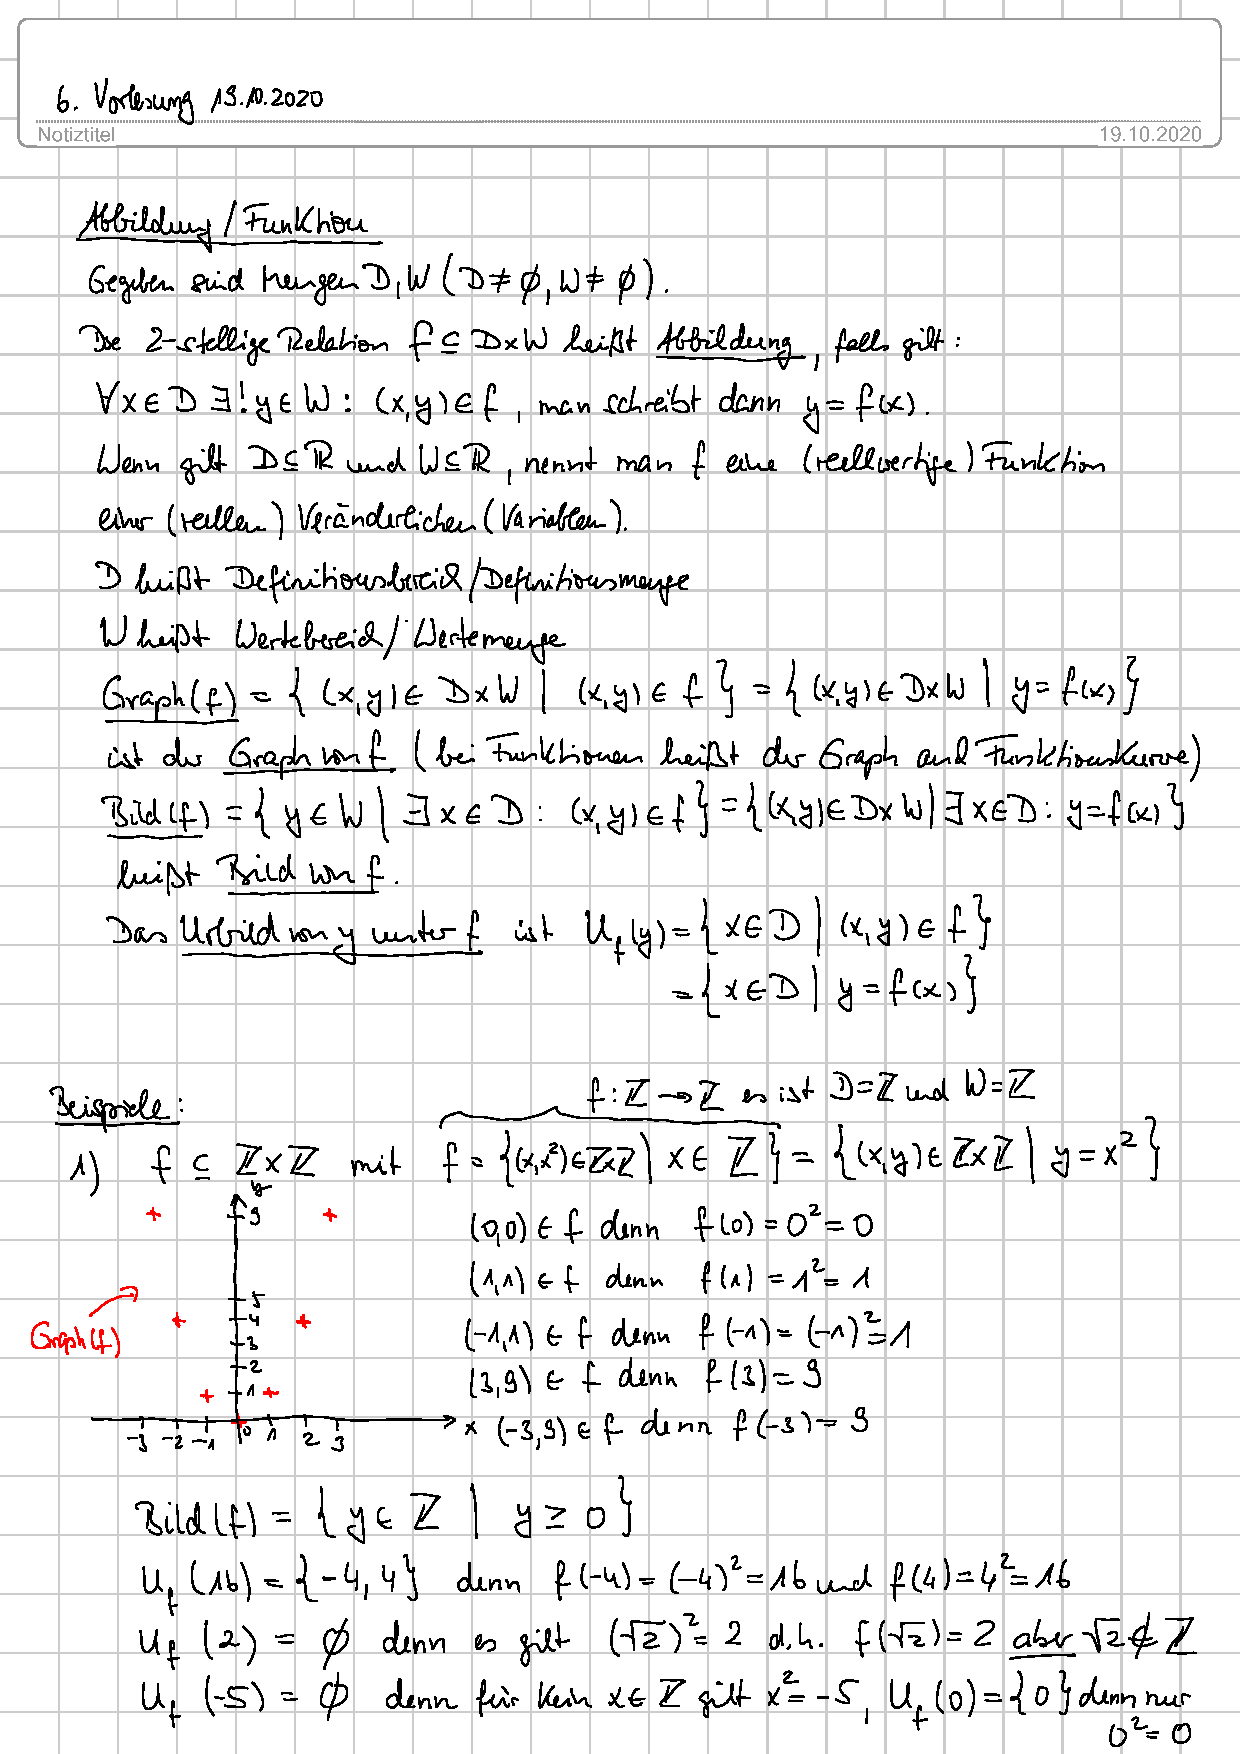
\includepdf[pages=-]{Mitschriften/6. Vorlesung 19.10.2020}

\section{Vorlesung 7 (20.10.2020)}
\subsection{Beipiele Vollständige Induktion}
\subsection{Definition durch Rekursion + Beispiele}
\subsection{Binomialkoeffizient}
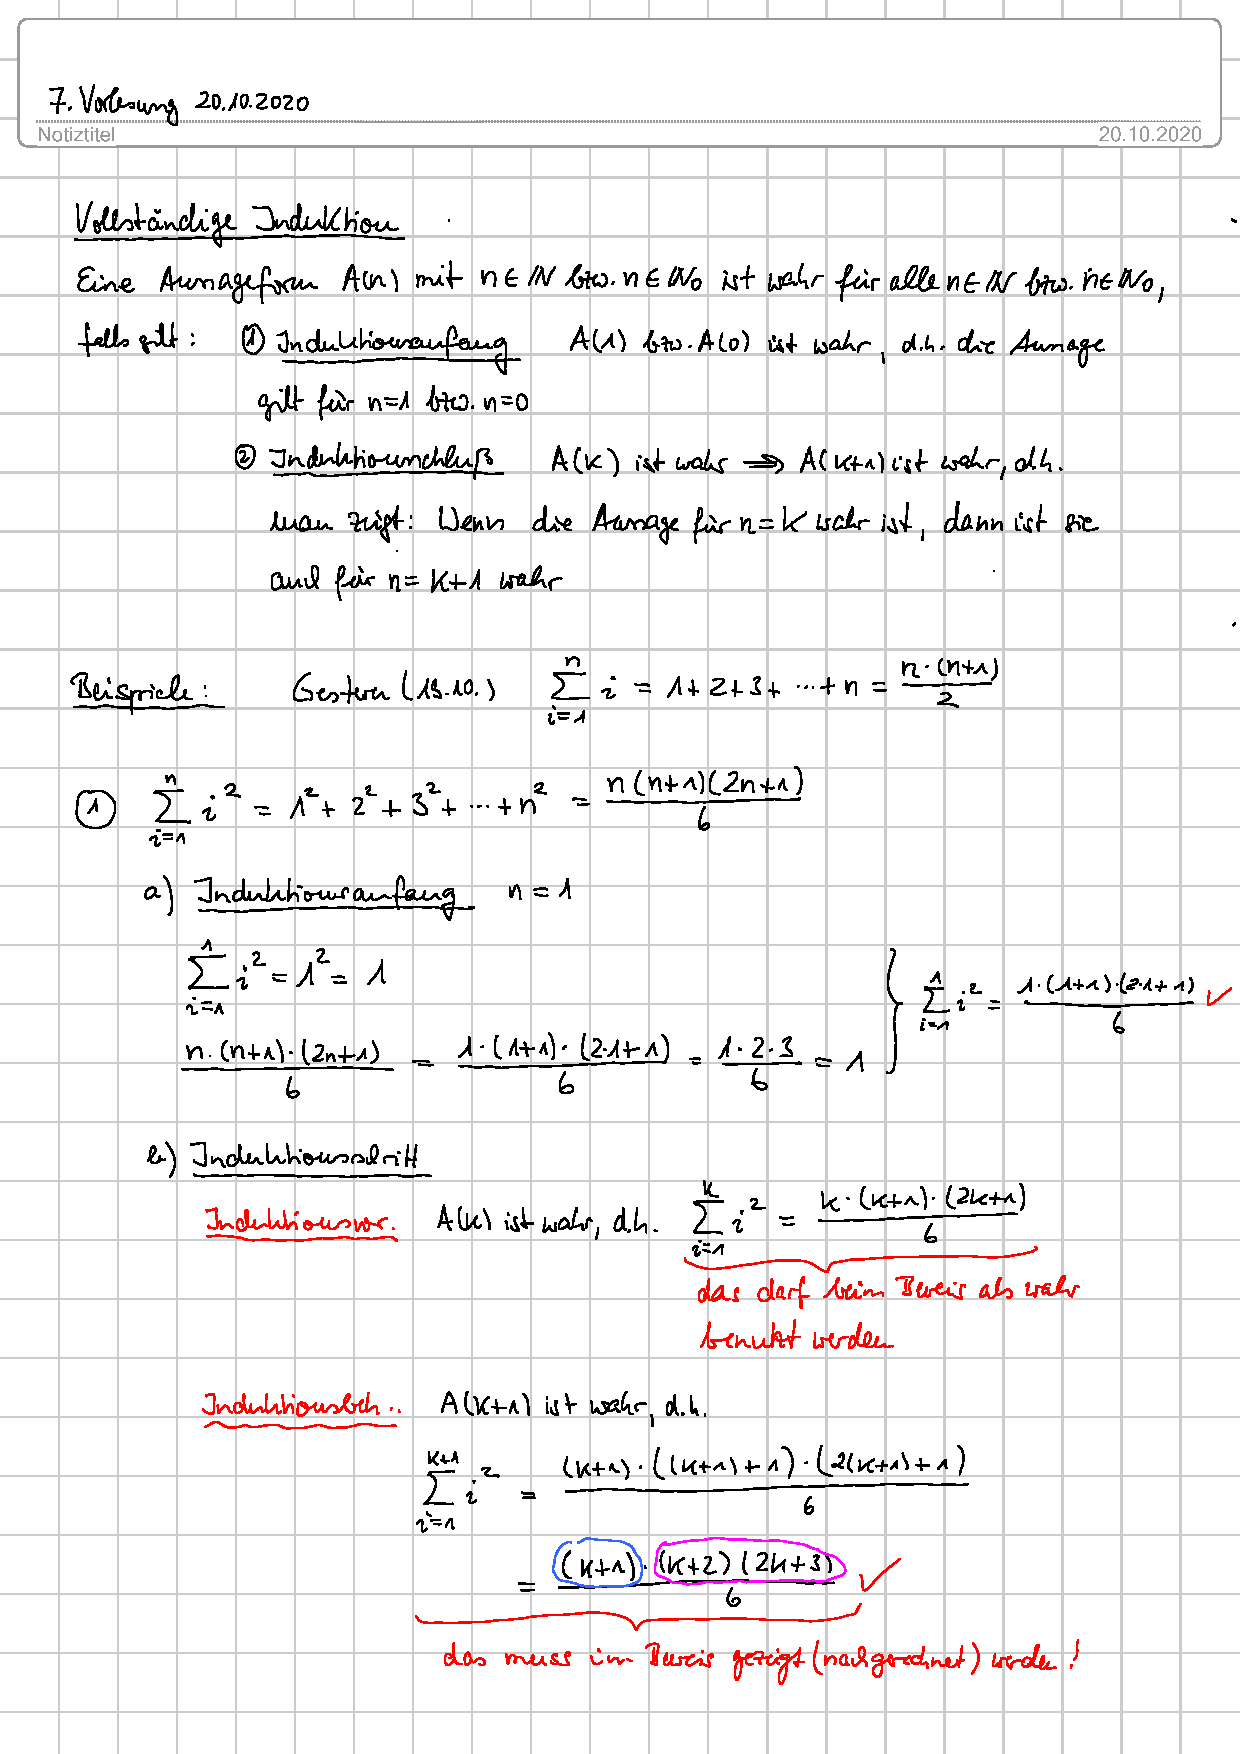
\includepdf[pages=-]{Mitschriften/7. Vorlesung 20.10.2020}

\section{Vorlesung 8 (21.10.2020)}
\subsection{Binomialkoeffizienten und Fakultät}
\subsection{Eigenschaften Binomialkoeffizient}
\subsection{Pascalsches Dreieck}
\subsection{1. Binomische Formel (+ 1. allgemeine Binomische Formel)}
\subsection{2. Binomische Formel (+ 2. allgemeine Binomische Formel)}
\subsection{Wiederholung: Ordnungsrelation, Vollständige Induktion}
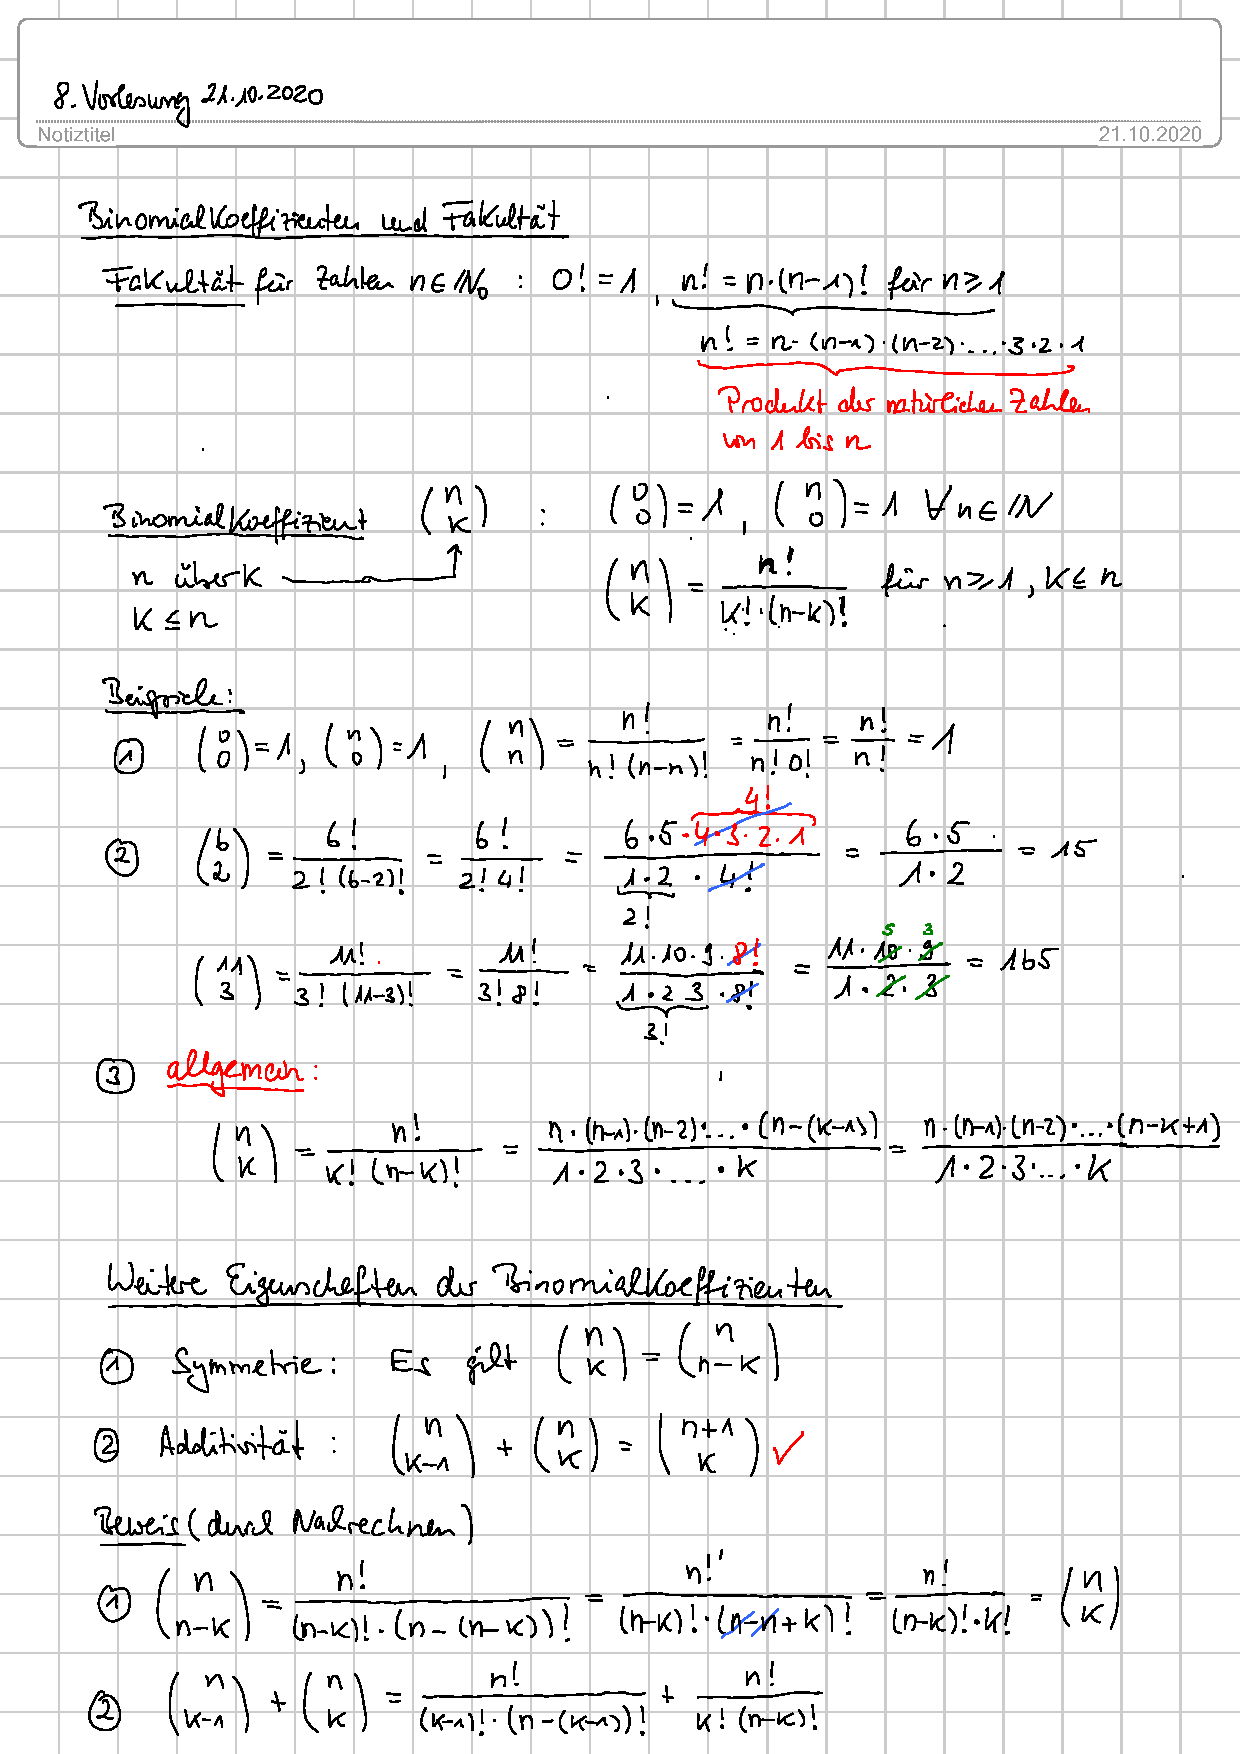
\includepdf[pages=-]{Mitschriften/8. Vorlesung 21.10.2020}

\section{Vorlesung 9 (26.10.2020)}
\subsection{Rechenregeln für Potenzen}
\subsection{3. Binomische Formel (+ 3. allgemeine Binomische Formel)}
\subsection{Elementares Multiplikationsprinzip}
\subsection{Elementare Kombinatorik (Anordnung, Auswahl)}
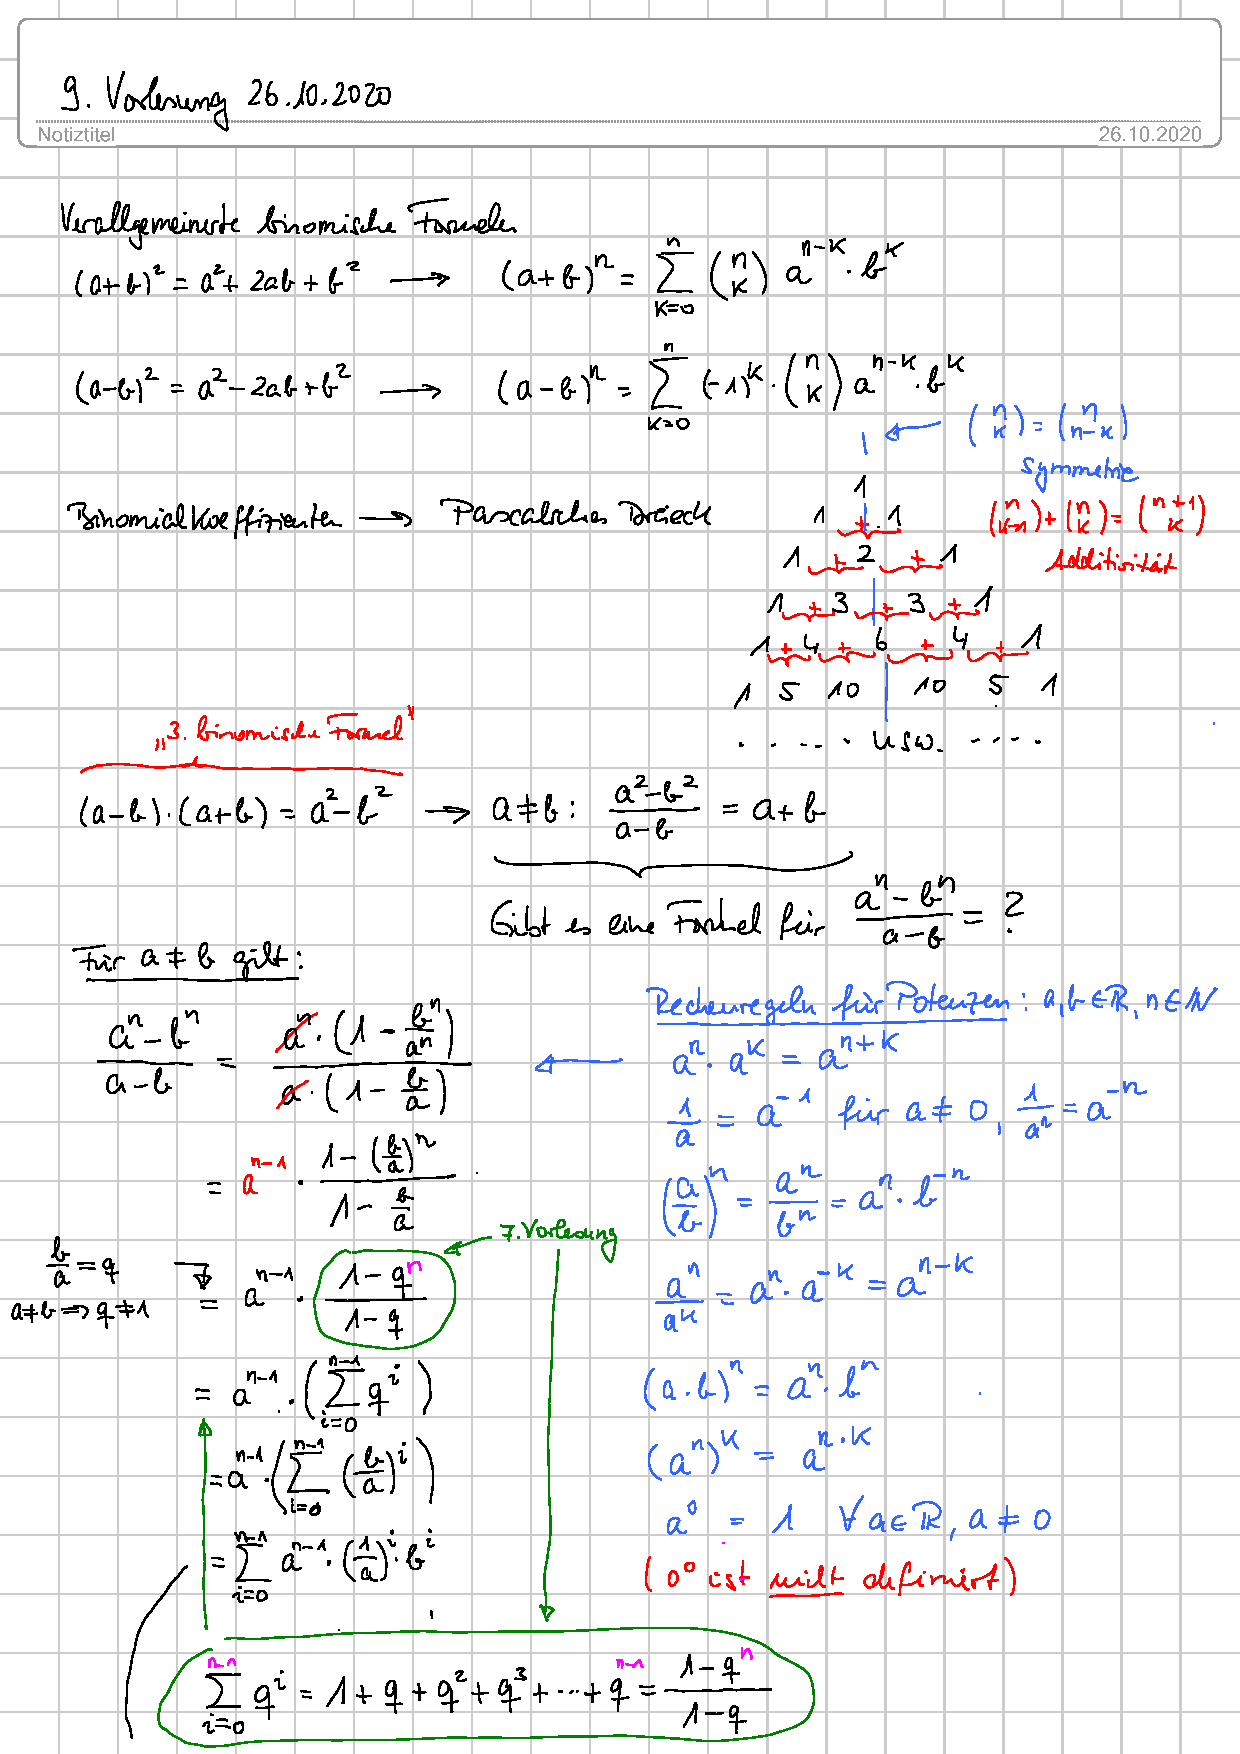
\includepdf[pages=-]{Mitschriften/9. Vorlesung 26.10.2020}

\section{Vorlesung 10 (27.10.2020)}
\subsection{Zusammenfassung Elementare Kombinatorik}
\subsection{Dezimaldarstellung rationaler Zahlen}
\subsection{Rechenregeln in den reellen Zahlen}
\subsection{Bemerkung: Was ist ein Körper, Anordnungsaxiom}
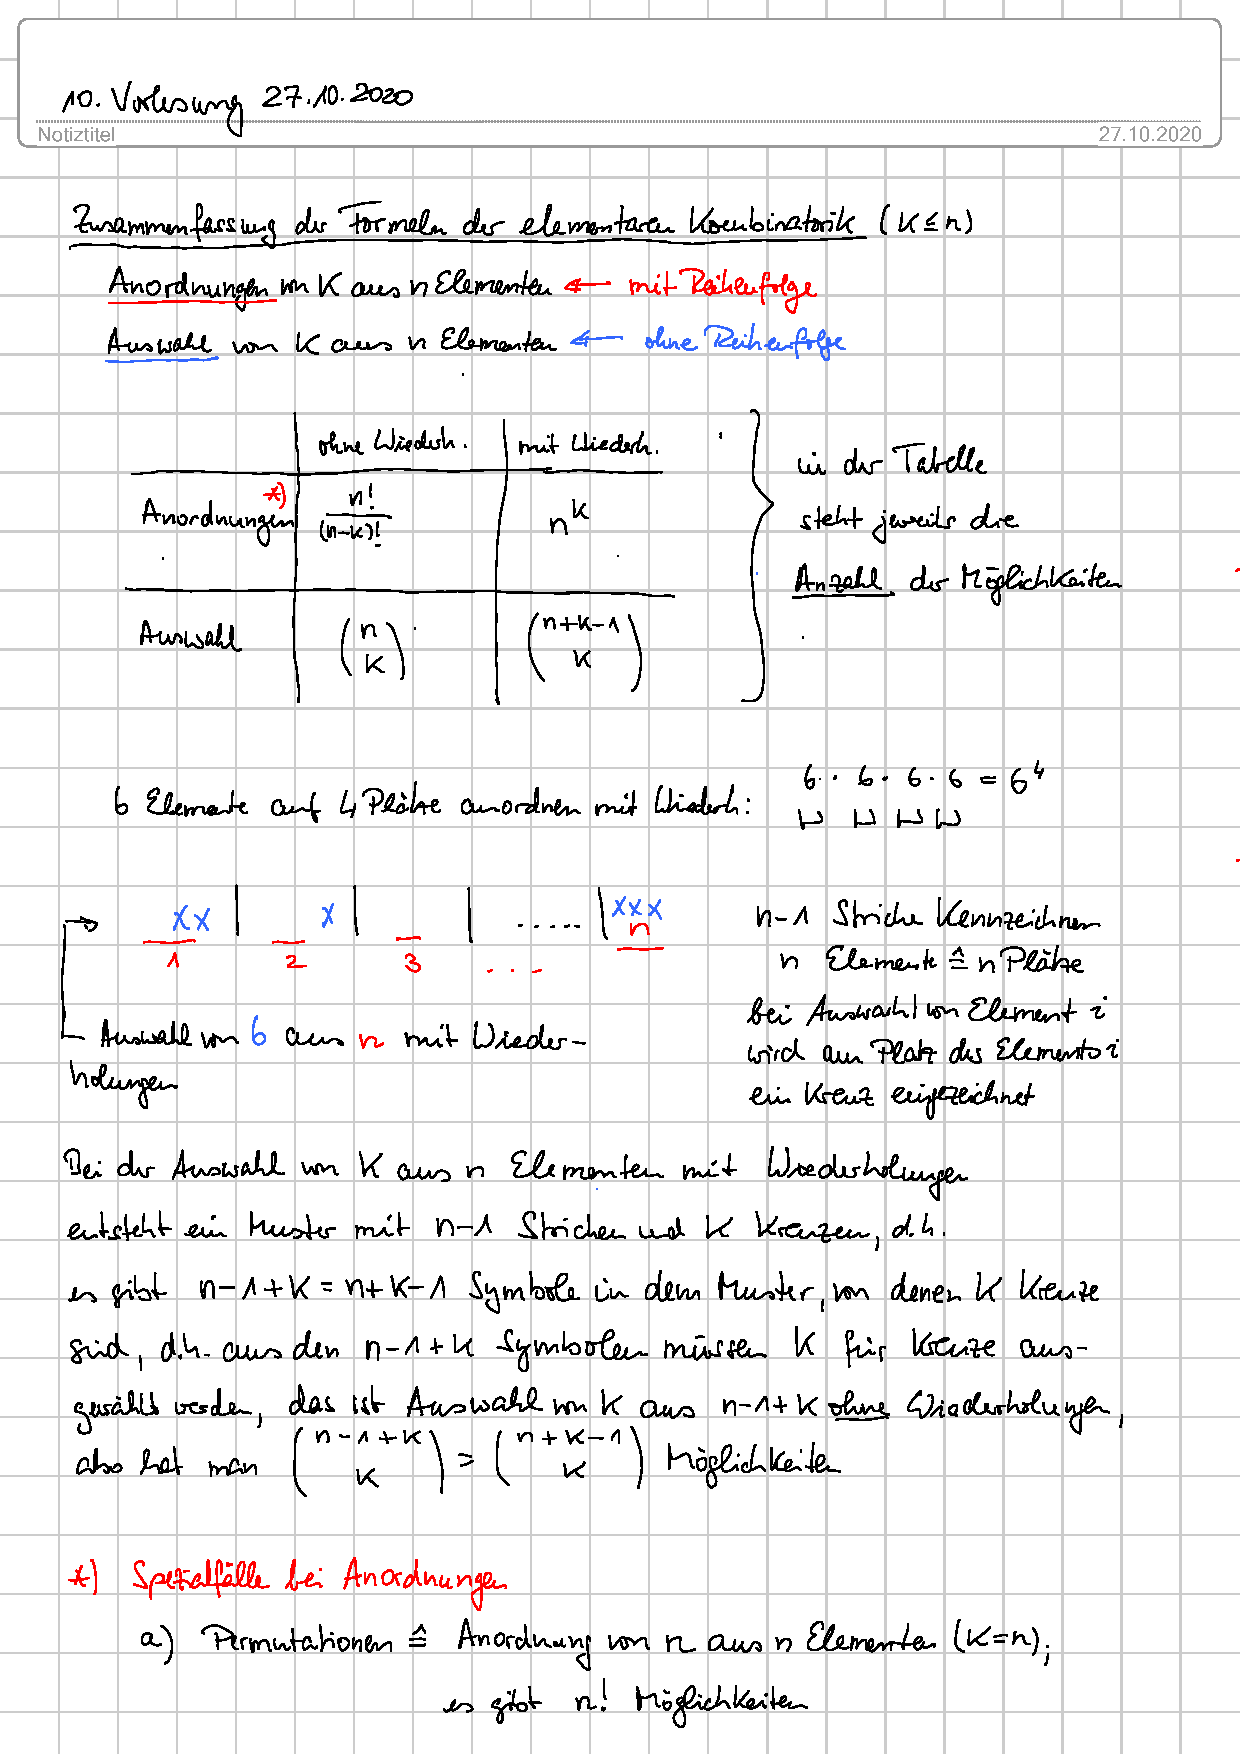
\includepdf[pages=-]{Mitschriften/10. Vorlesung 27.10.2020}

\section{Vorlesung 11 (28.10.2020)}
\subsection{Rechenregeln der Anordnung}
\subsection{Intervalle als Mengen}
\subsection{unendlich-Symbol}
\subsection{Definition: Term}
\subsection{Definition: Betrag einer reellen Zahl}
\subsection{erste Rechenregeln für den Betrag}
\subsection{Betrag, Ungleichung und Intervalle}
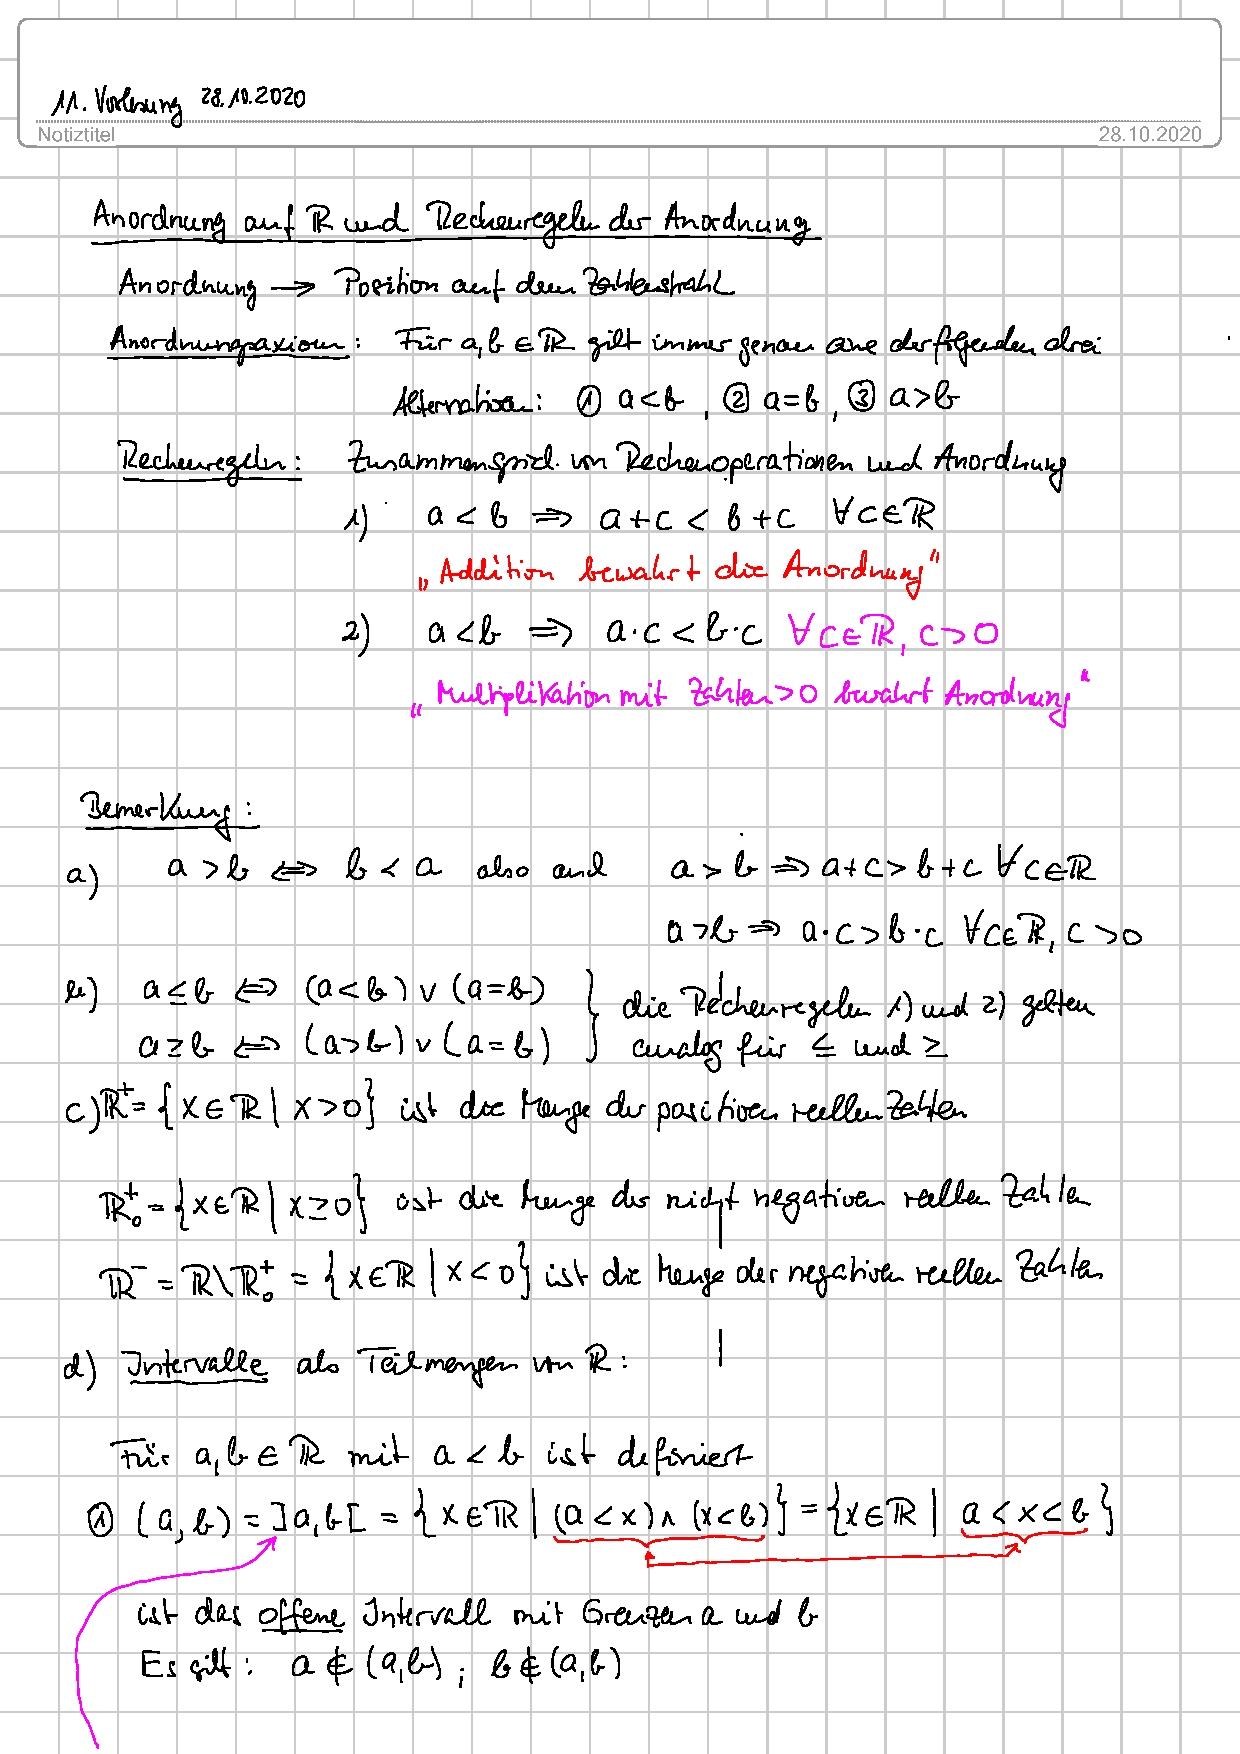
\includepdf[pages=-]{Mitschriften/11. Vorlesung 28.10.2020}

\section{Vorlesung 12 (02.11.2020)}
\subsection{Anordnung, Ungleichung und Intervalle}
\subsection{Potenzen und Wurzeln in den reellen Zahlen}
\subsection{Rechenregeln für Wurzeln}
\subsection{Quadratische Gleichungen und Ungleichungen in den reellen Zahlen}
\subsection{pq-Formel}
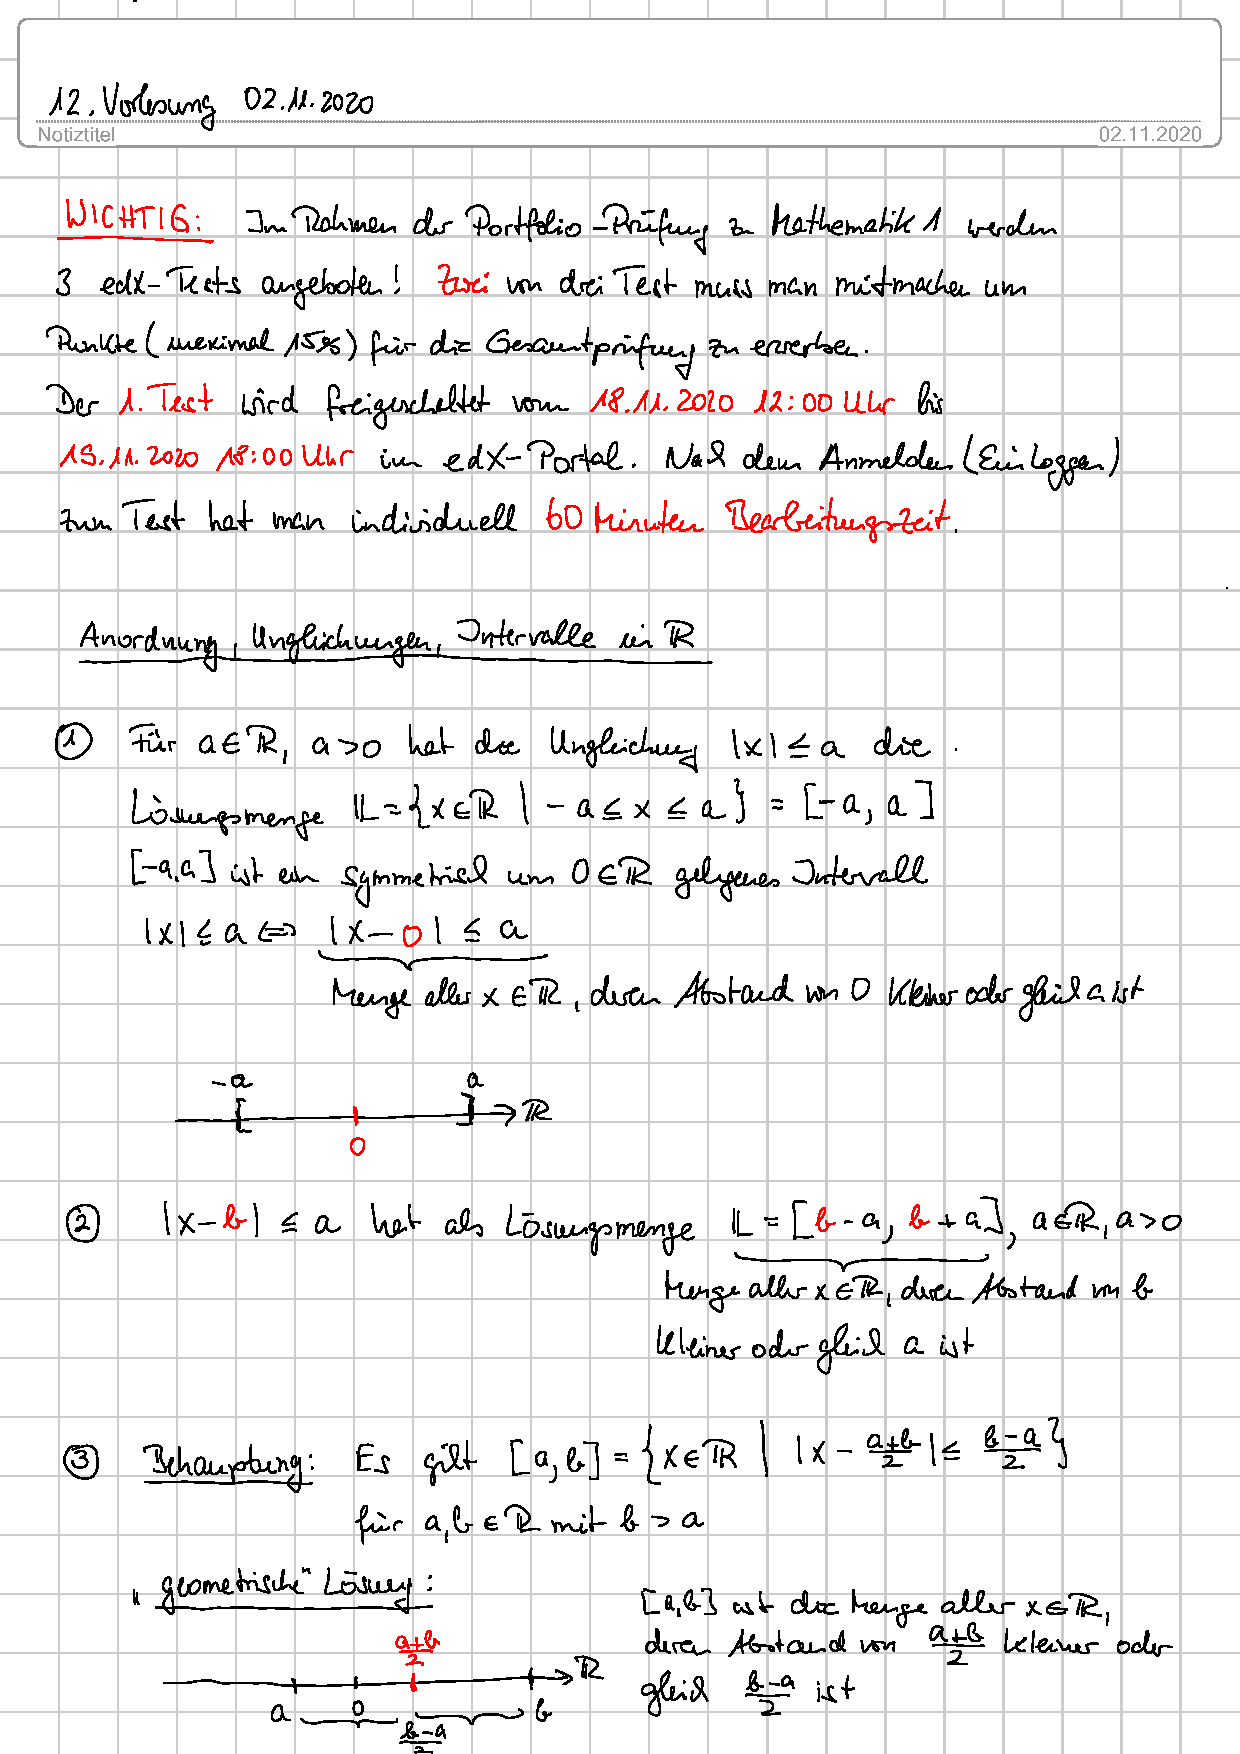
\includepdf[pages=-]{Mitschriften/12. Vorlesung 02.11.2020}

\section{Vorlesung 13 (03.11.2020)}
\subsection{Linearfaktoren des quadratischen Polynoms}
\subsection{Mitternachtsformel}
\subsection{Quadratische Ungleichungen}
\subsection{Definition: Logarithmus}
\subsection{Rechenregeln für Logarithmen}
\subsection{Zahldarstellungen (umrechnung)}
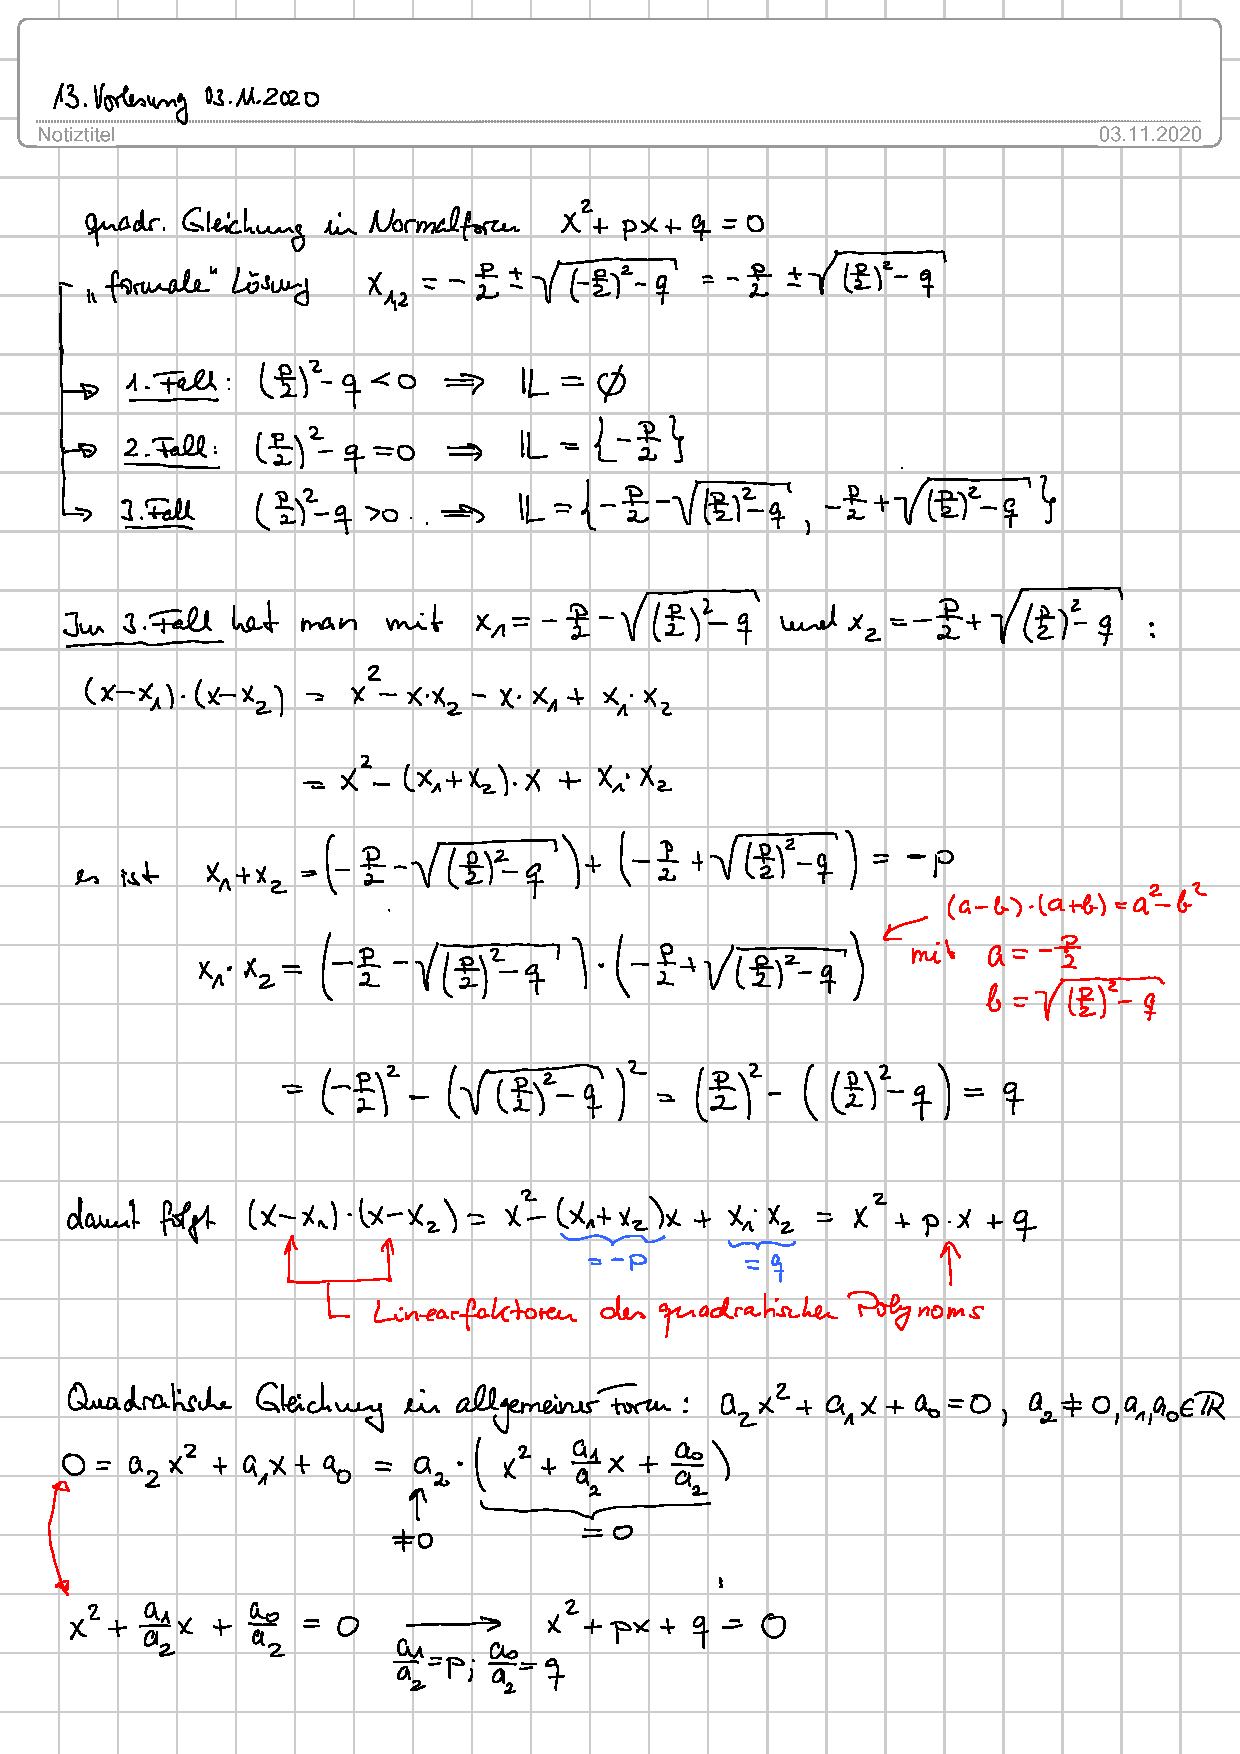
\includepdf[pages=-]{Mitschriften/13. Vorlesung 03.11.2020}

\section{Vorlesung 14 (04.11.2020)}
\subsection{Beispiel: Zahldarstellungen (umrechnung)}
\subsection{Brüche in anderen Zahldarstellungen}
\subsection{Zweiter Blick auf Ungleichungen und Betrag}
\subsection{Rechenregeln für den Betrag}
\subsection{Beweisidee Dreiecksungleichung}
\subsection{Definition: Verknüfungen auf Mengen}
\subsection{Definition: Gruppe, Halbgruppe, abelsche Gruppe}
\subsection{Definition: Ring, Ring mit Eins, Kommutativer Ring mit Eins}
\subsection{Definition: Körper}
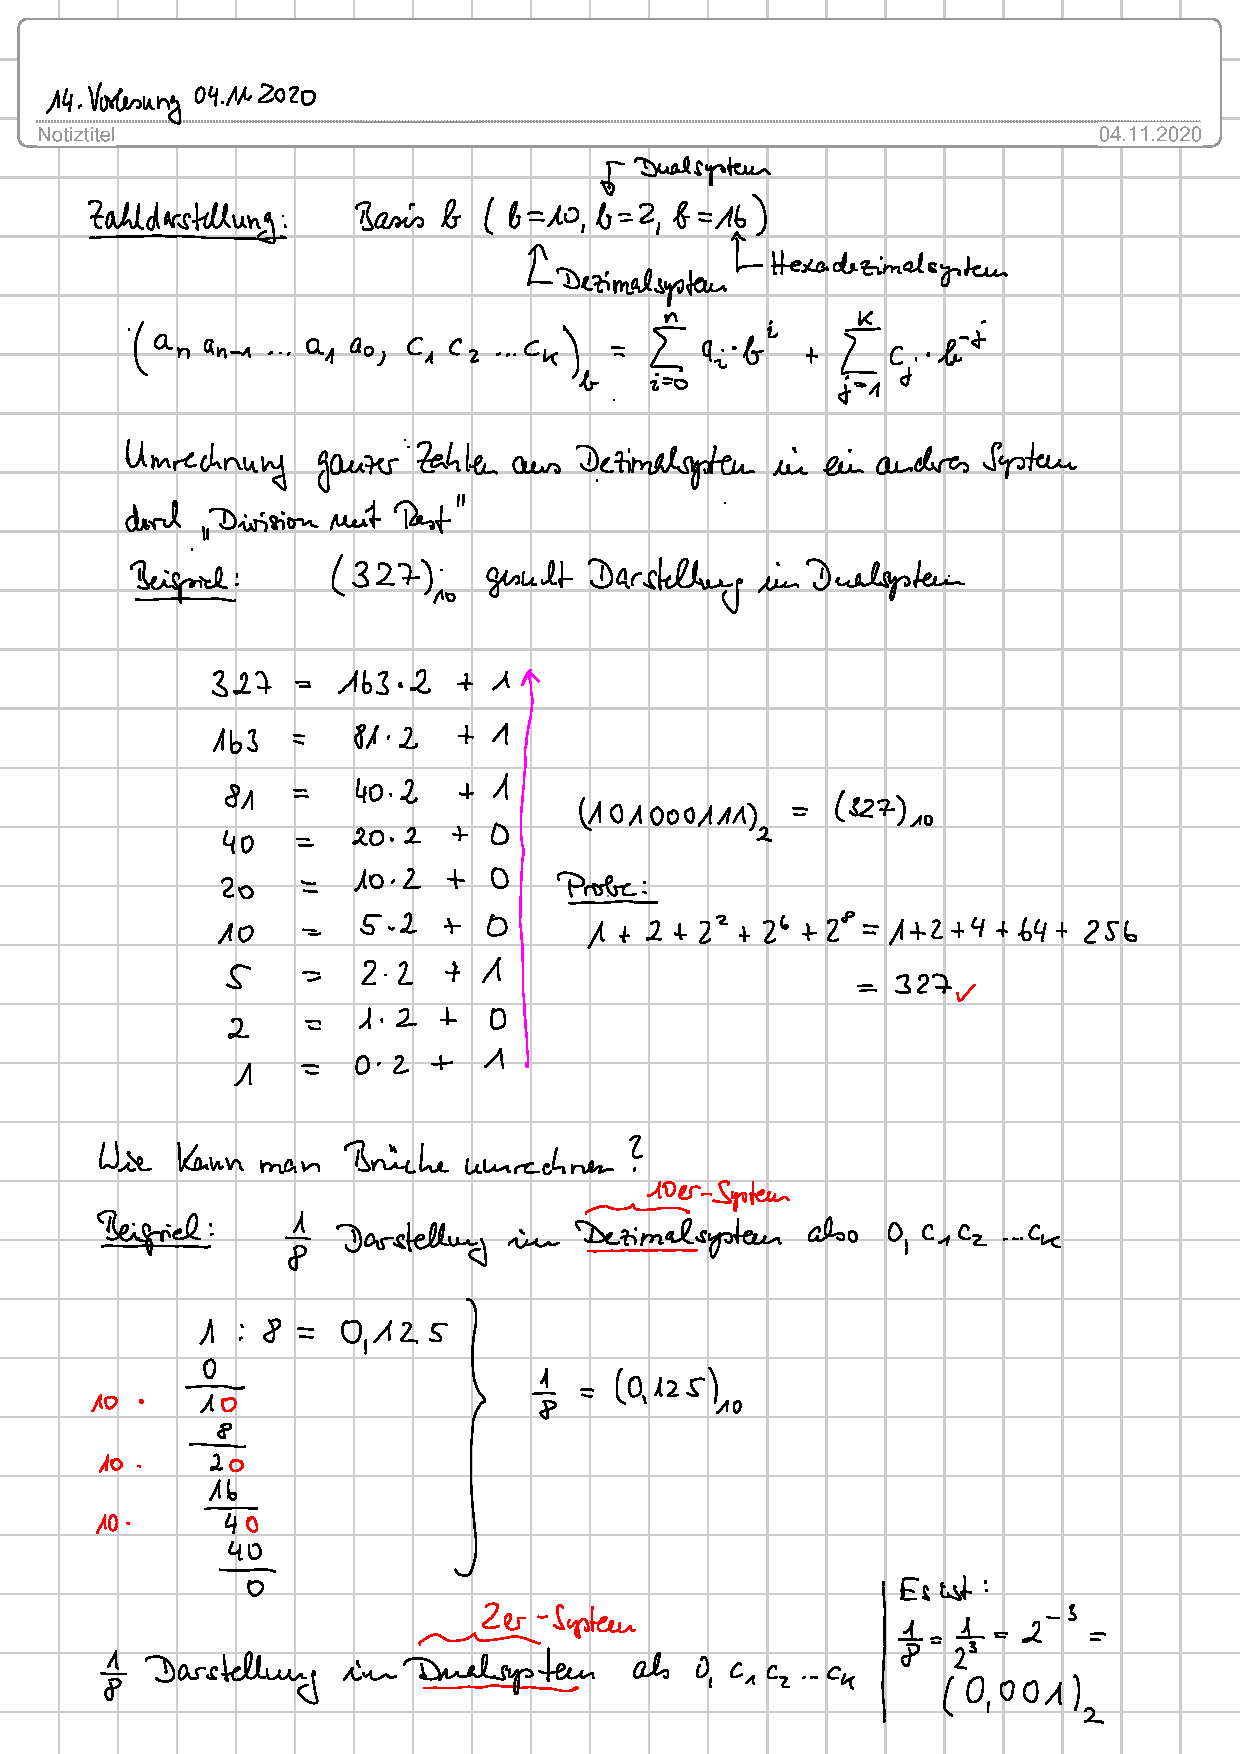
\includepdf[pages=-]{Mitschriften/14. Vorlesung 04.11.2020}

\section{Vorlesung 15 (16.11.2020)}
\subsection{5 Körperaxiome + Beispiele}
\subsection{Definition: Ganzzahlige Teiler}
\subsection{Definition: Primzahl}
\subsection{Definition: Gemeinsame Teiler / Größter gemeinsamer Teiler}
\subsection{Division mit Rest}
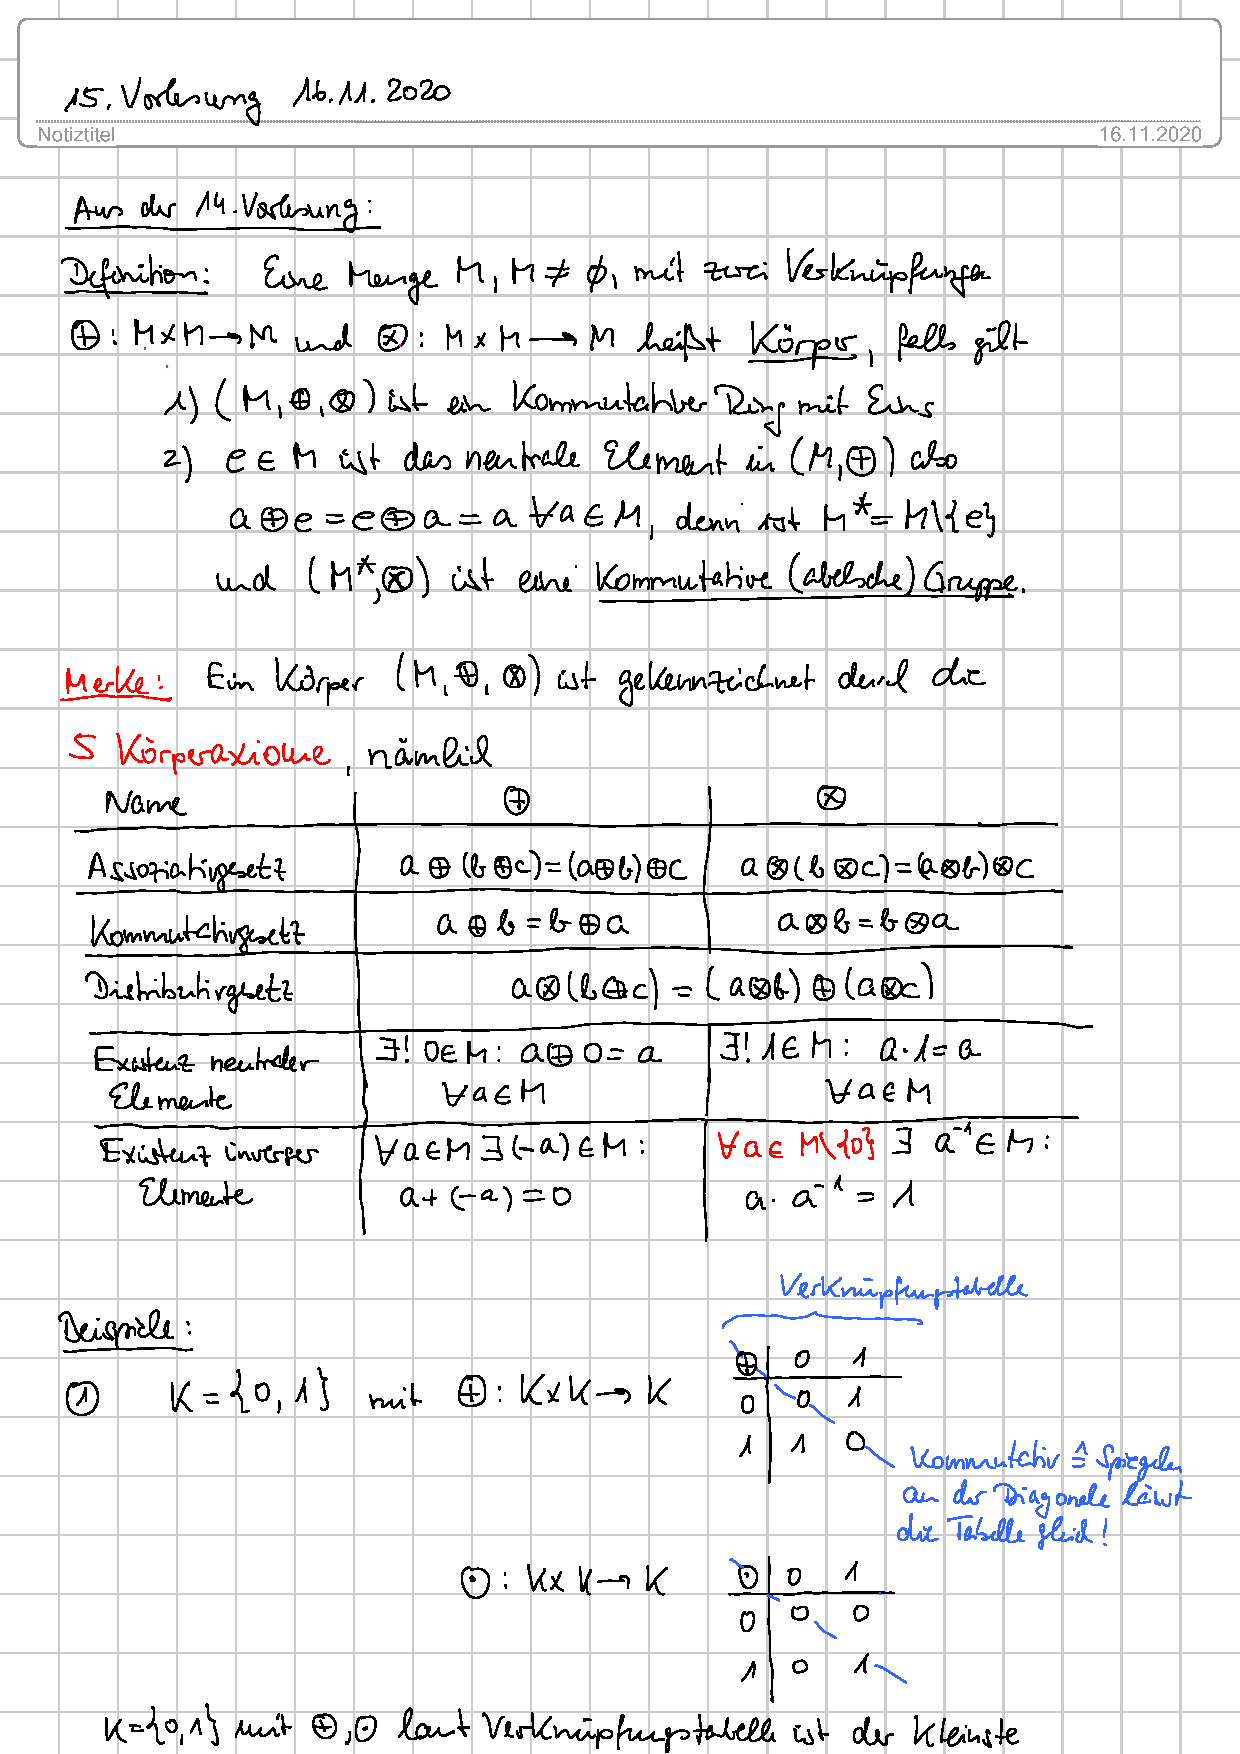
\includepdf[pages=-]{Mitschriften/15. Vorlesung 16.11.2020}

\section{Vorlesung 16 (17.11.2020)}
\subsection{Wiederholung Teilermengen, Primzahl, gemeinsame Teiler}
\subsection{Definition: ggT, Division mit Rest, Teilerfremd}
\subsection{Beweis: Division mit Rest}
\subsection{Euklidischer Algorithmus}
\subsection{Lemma von Bézout}
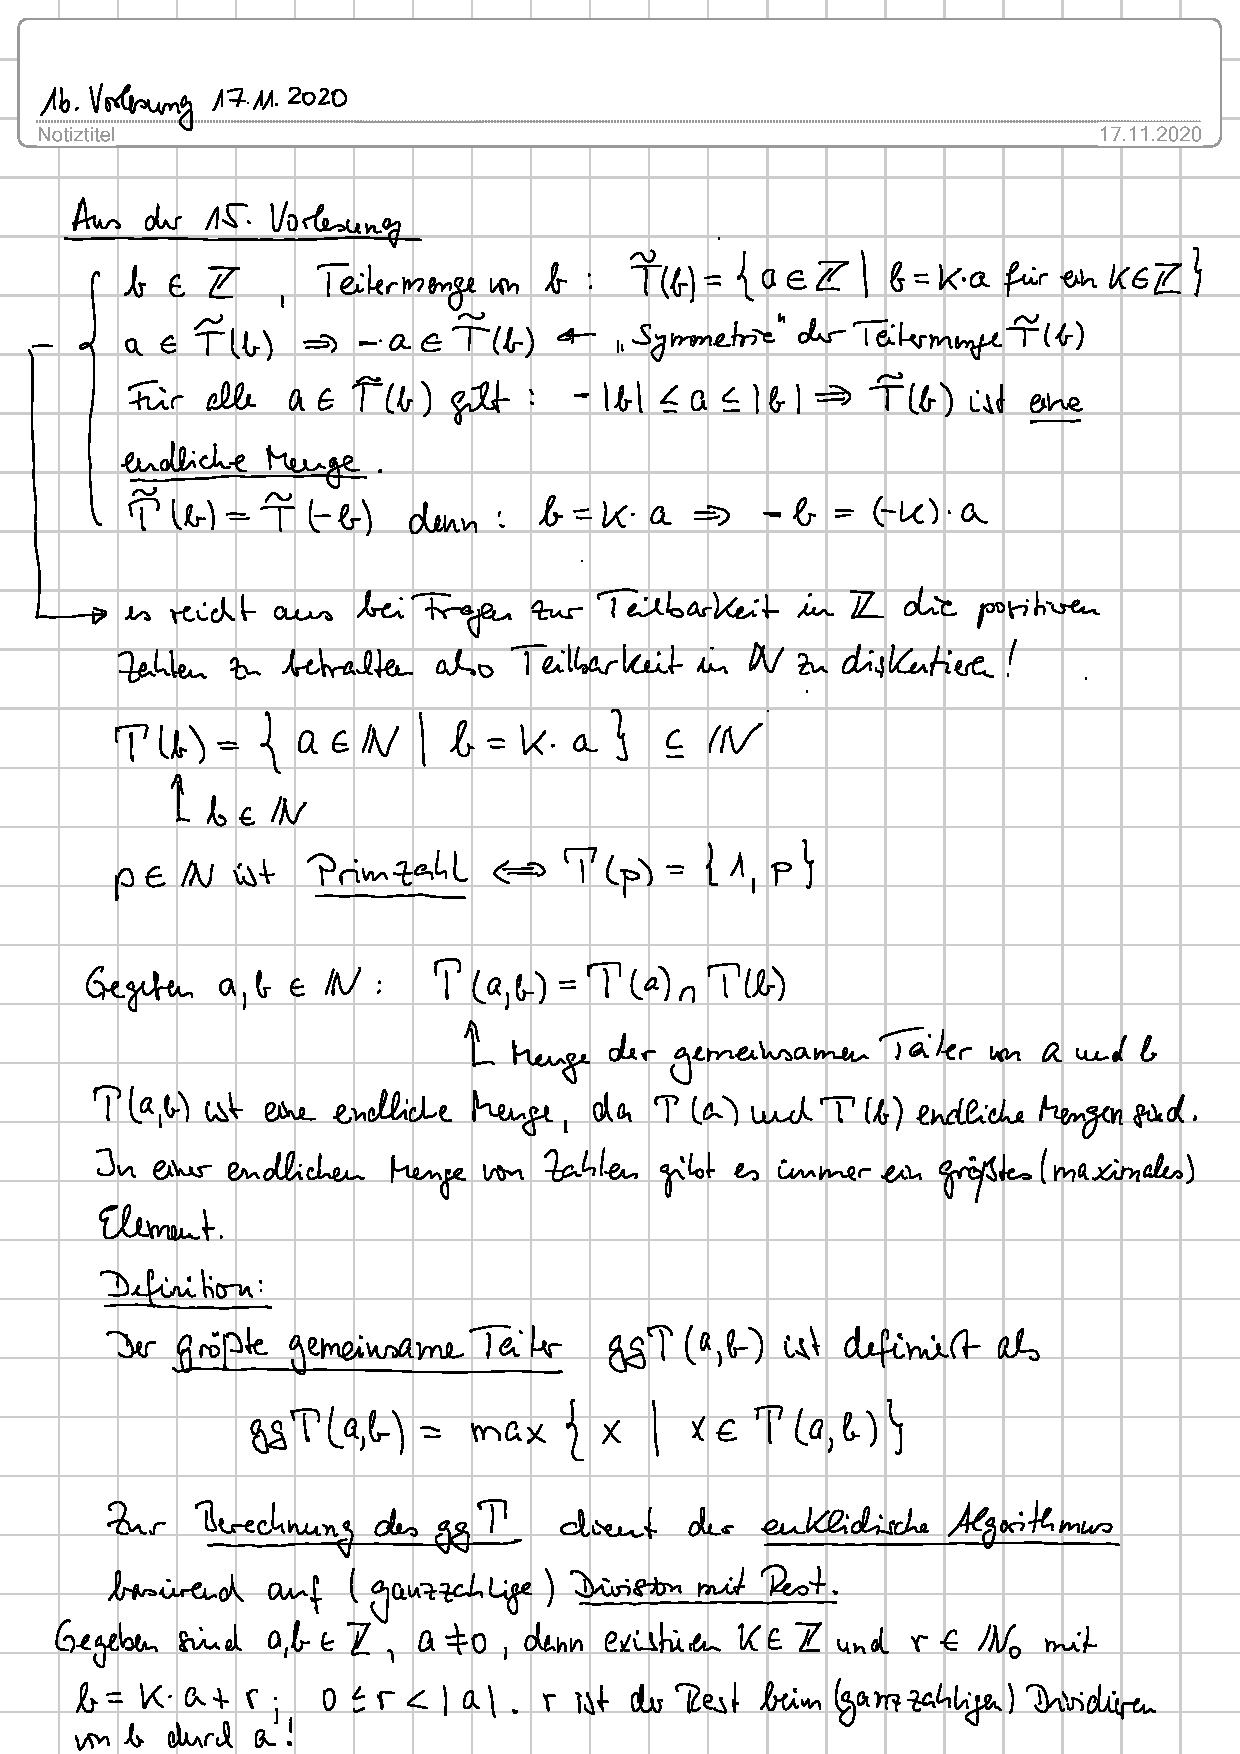
\includepdf[pages=-]{Mitschriften/16. Vorlesung 17.11.2020}


\section{Vorlesung 17 (18.11.2020)}
\subsection{Teilen mit Rest}
\subsection{Teilen und Äquivalenzrelationen, Restemengen}
\subsection{Rechenoperationen in $Z_m$, Körper?, kommutativer Ring mit Eins?}
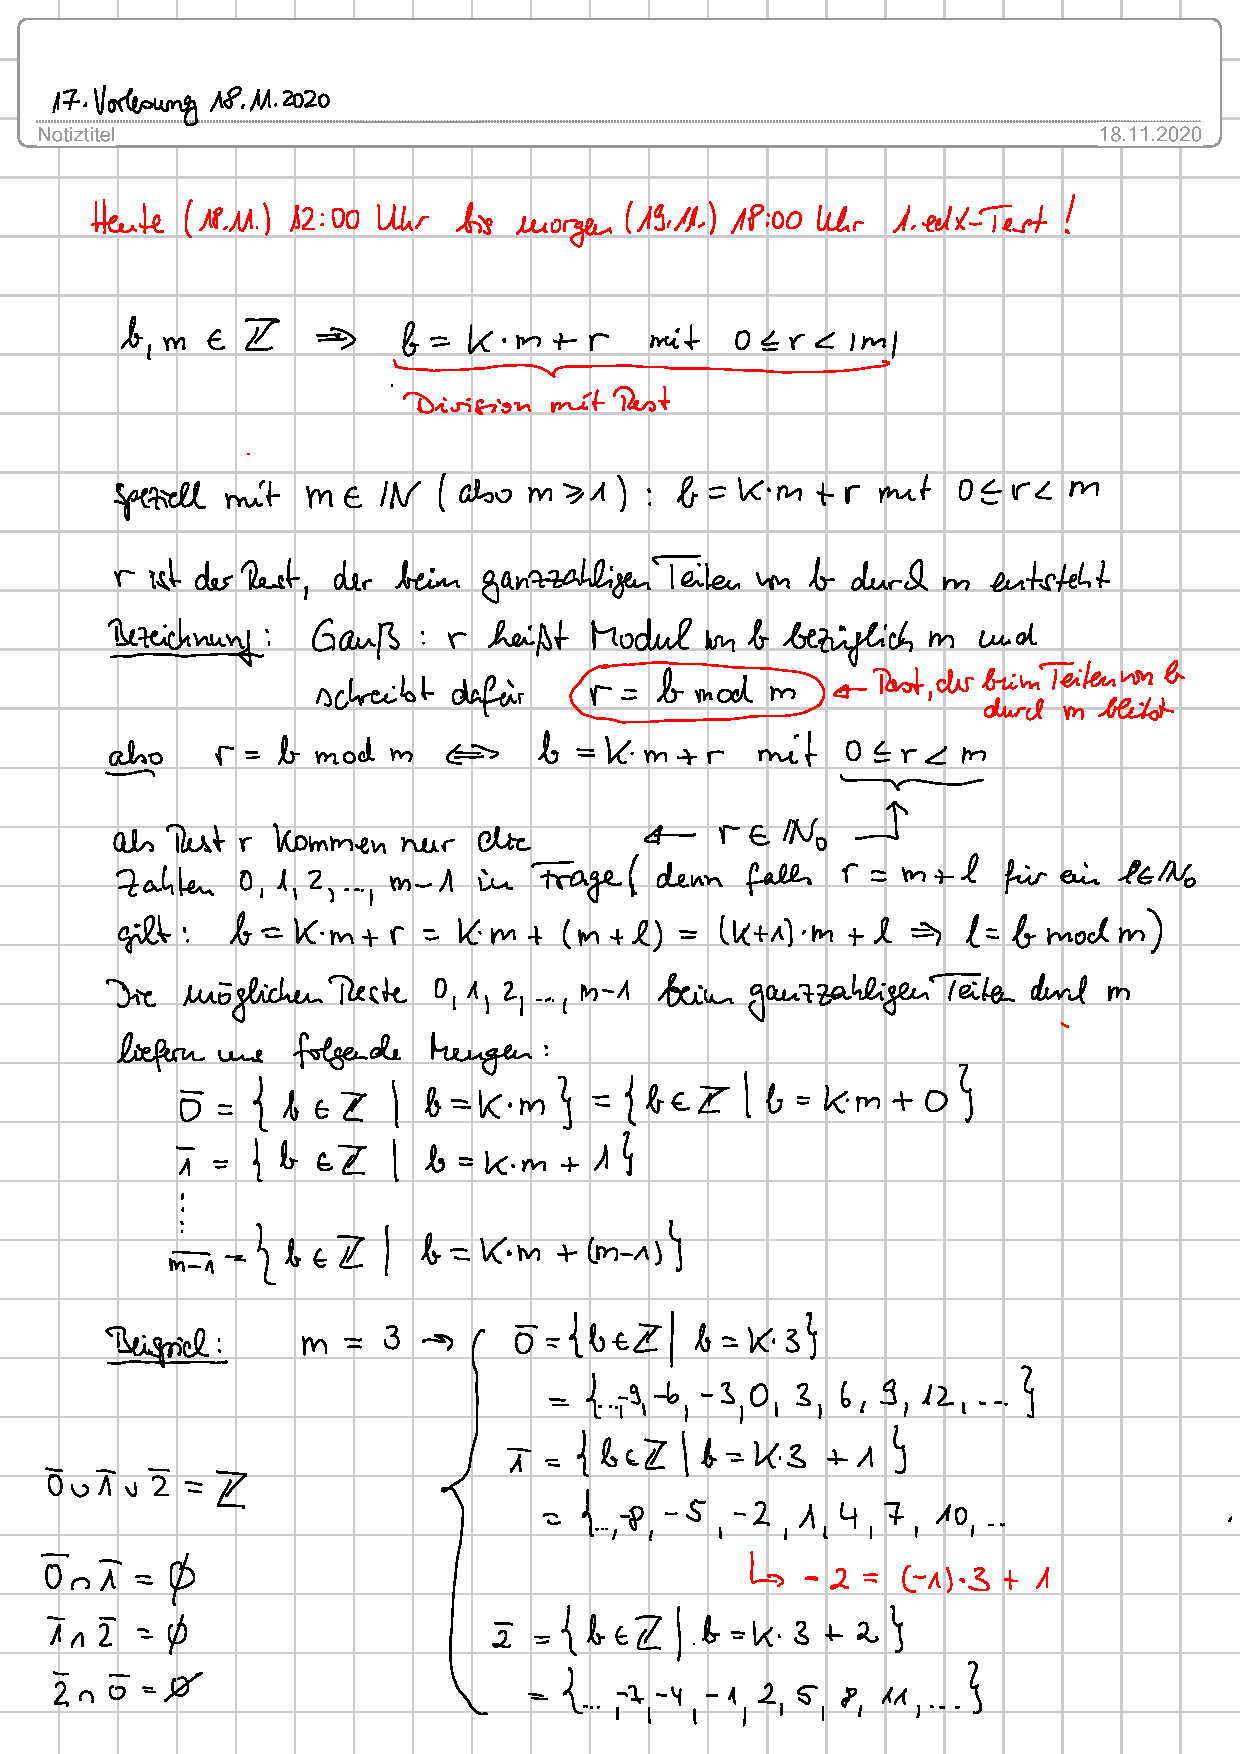
\includepdf[pages=-]{Mitschriften/17. Vorlesung 18.11.2020}

\section{Vorlesung 18 (23.11.2020)}
\subsection{Restklassen mit Primzahlen sind Körper + Beispiel}
\subsection{simultane Kongruenzen}
\subsection{chinesischer Restsatz}
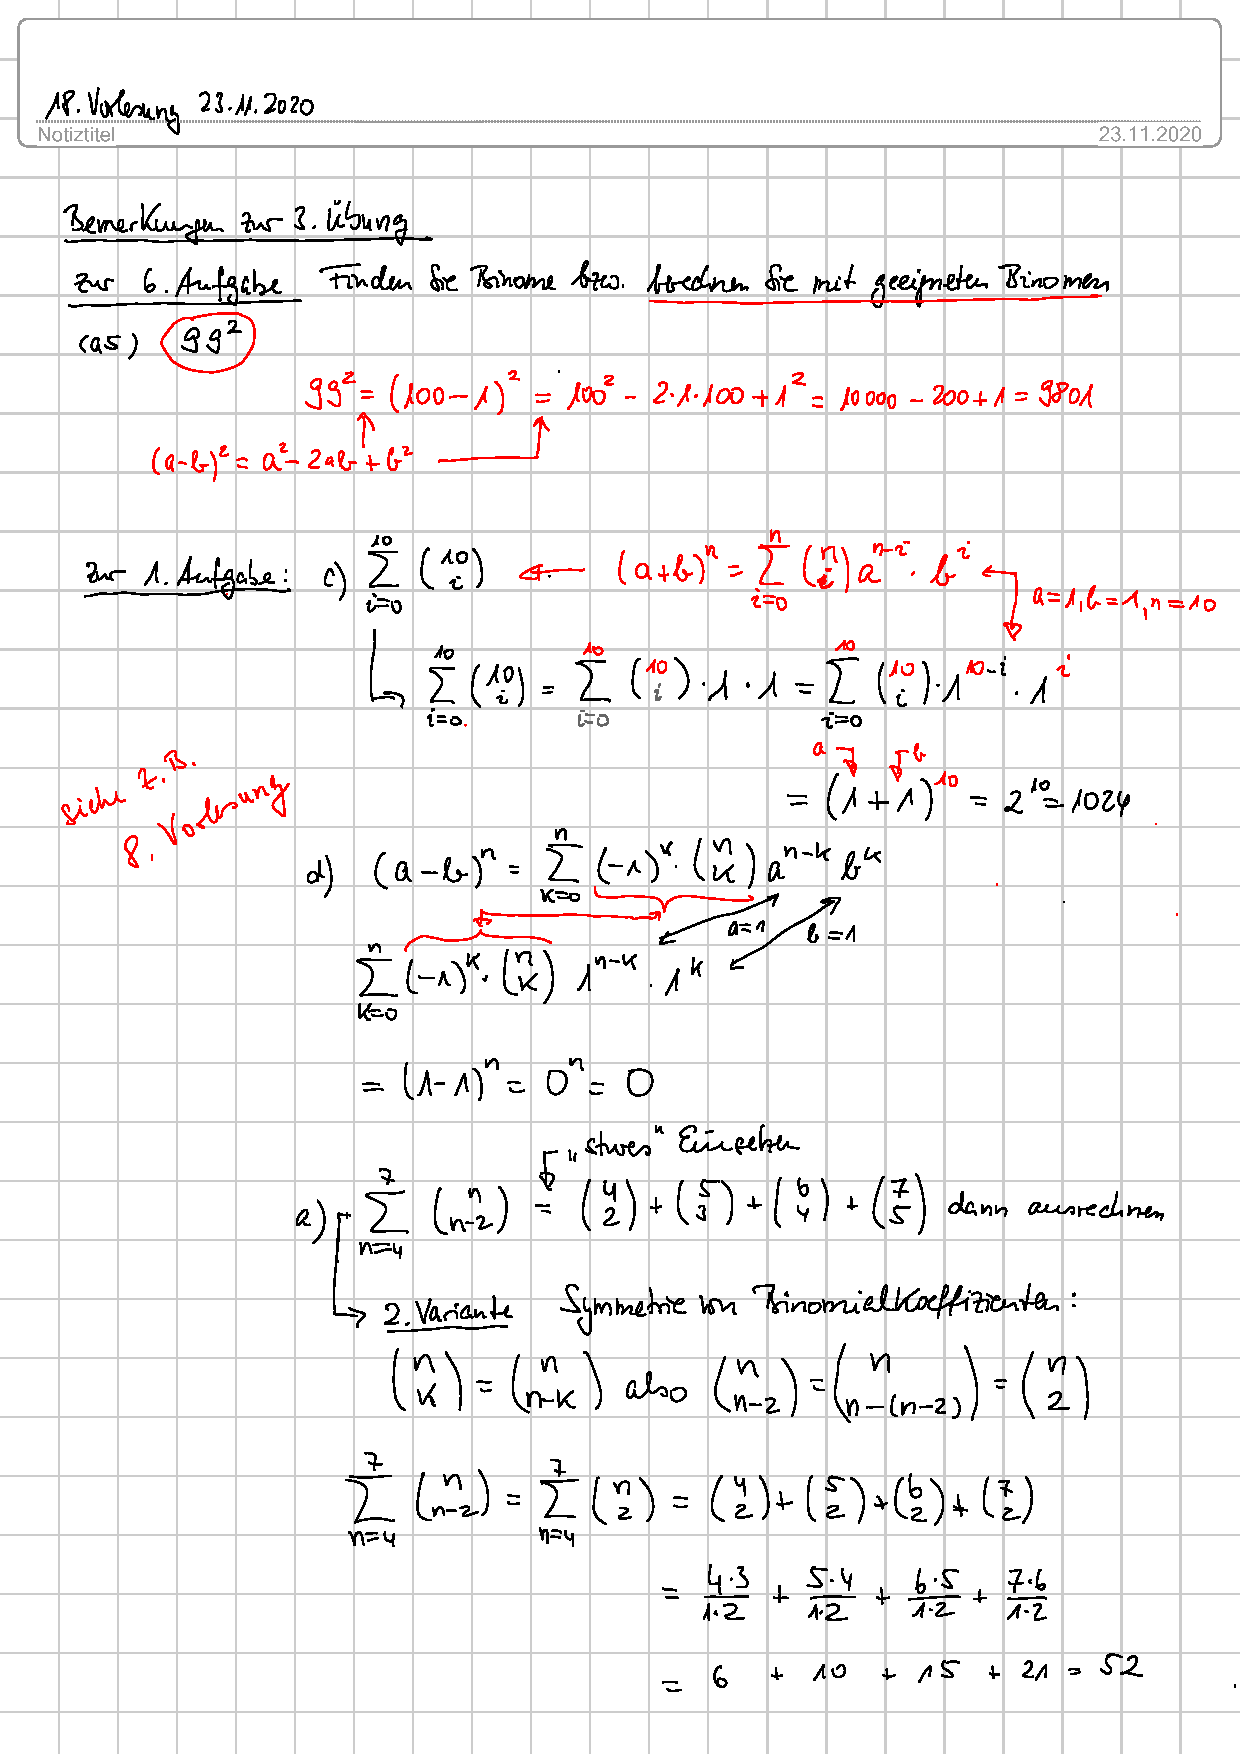
\includepdf[pages=-]{Mitschriften/18. Vorlesung 23.11.2020}

\section*{Vorlesung 19 (24.11.2020)}
\subsection*{Chinesischer Restsatz: Beweis, Beispiel}
\subsection*{Allgemeiner chinesischer Restsatz}
\subsection*{RSA: Anwendung von modularer Arithmetik}
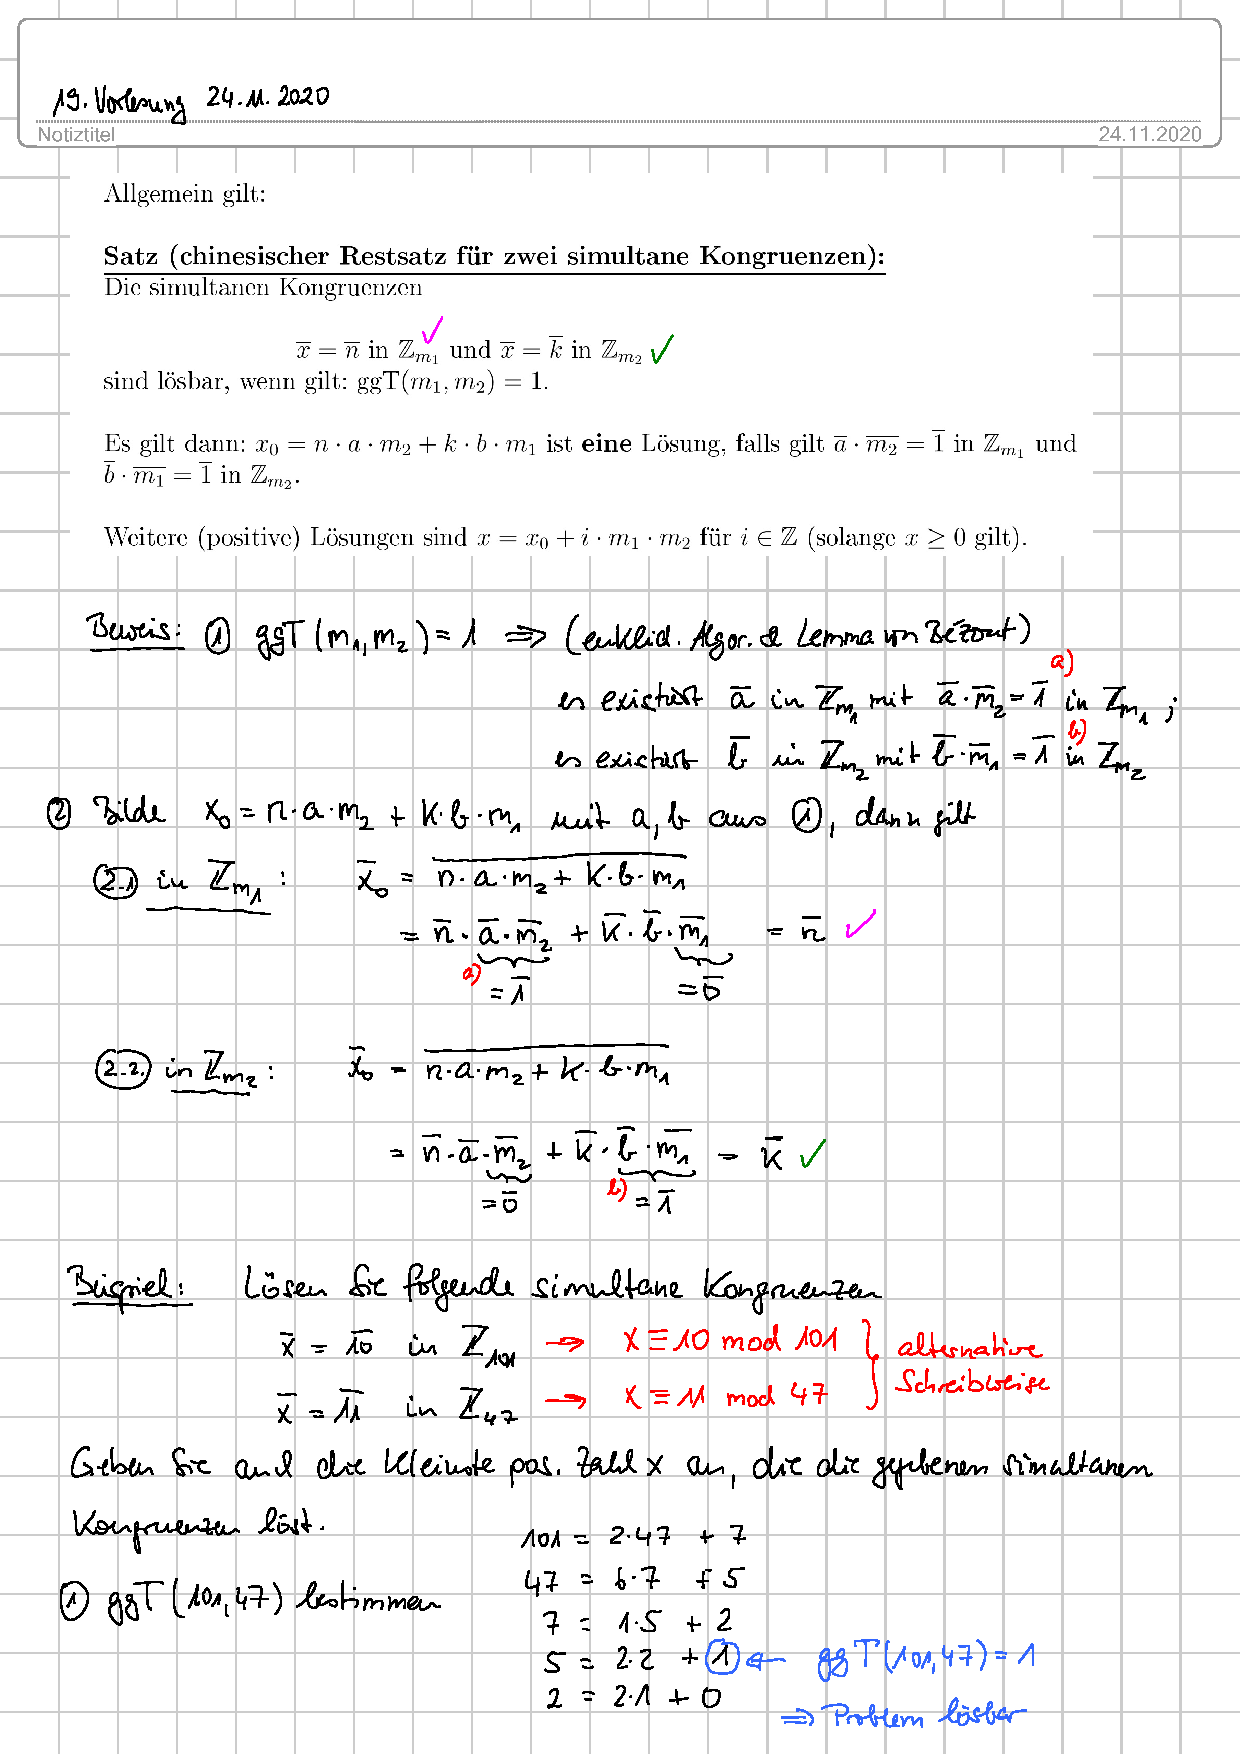
\includepdf[pages=-]{Mitschriften/19. Vorlesung 24.11.2020}

\section*{Vorlesung 20 (25.11.2020)}
\subsection*{Prinzip der RSA-Verschlüsselung}
\subsection*{Eulersche-phi-Funktion}
\subsection*{Satz von Euler}
\subsection*{'kleiner' Satz von Fermat}
\subsection*{Beweis: RSA-Algorithmus}
\subsection*{Beweis: Satz von Euler}
\subsection*{Einführung: Lineare Gleichungssysteme}
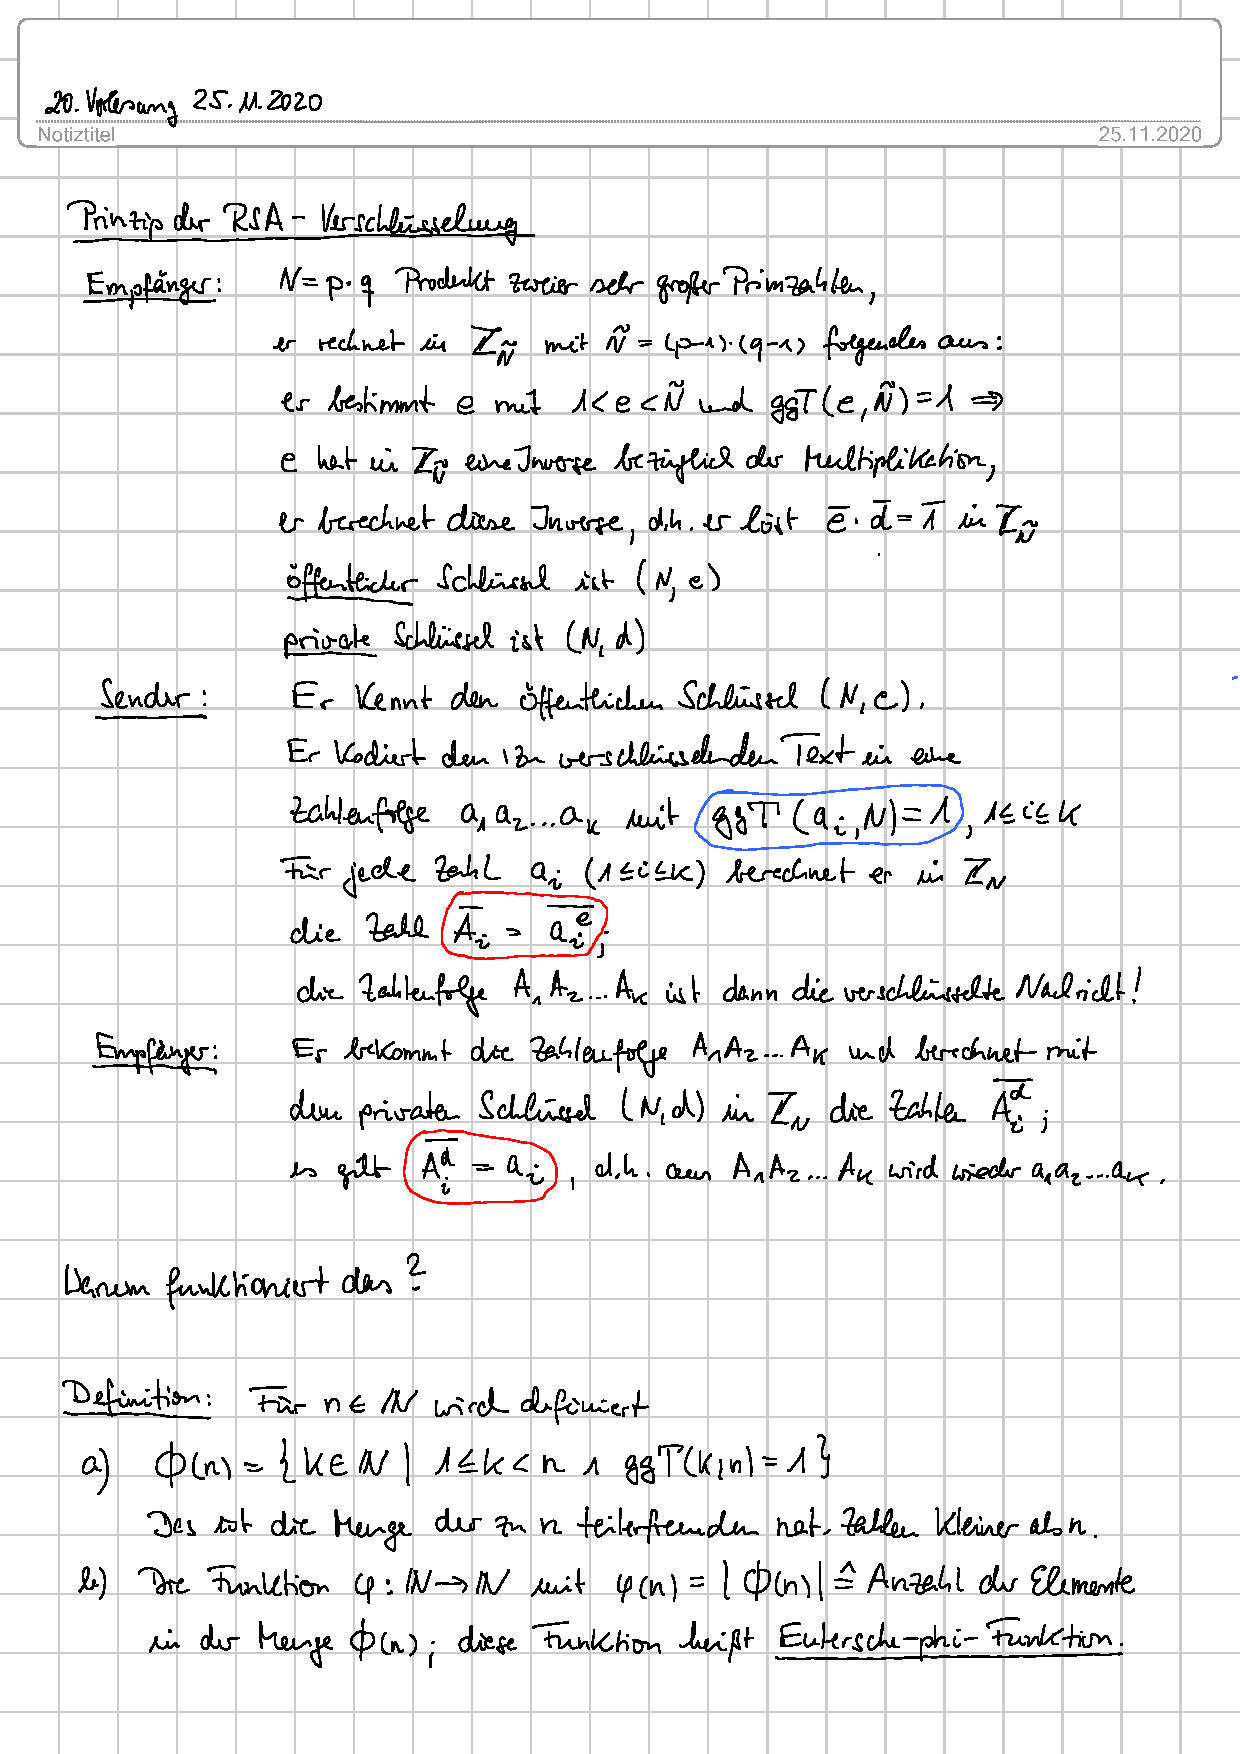
\includepdf[pages=-]{Mitschriften/20. Vorlesung 25.11.2020}


\end{document}